%==============================================================================
%  Trabalho Final — Teoria da Informação (TIP7266 / PPGETI-UFC) — 2026.1
%  Caracterização Informacional do Envelhecimento e do Ruído em Sensores
%  de Slack Embarcados — versão em português de main.tex
%
%  Build:  pdflatex main_pt && bibtex main_pt && pdflatex main_pt && pdflatex main_pt
%  (ou simplesmente: latexmk -pdf main_pt.tex)
%
%  Esta é uma tradução do documento em inglês (main.tex): mesmos macros de
%  notação, mesmos números gerados pelo pipeline (generated/values.tex),
%  mesmas figuras e mesma bibliografia -- apenas o texto corrido, em
%  sections_pt/ e tables_pt/, está em português. Ver CLAUDE.md /
%  05_Execution_Plan.md para o contrato de reprodutibilidade.
%==============================================================================
\documentclass[11pt,a4paper]{article}

\usepackage[utf8]{inputenc}
\usepackage[T1]{fontenc}
\usepackage[brazilian]{babel}
\usepackage[margin=1in]{geometry}

% --- math ---
\usepackage{amsmath,amssymb,amsfonts}
\usepackage{bm}

% --- tables / figures ---
\usepackage{booktabs}
\usepackage{graphicx}
\graphicspath{{figures/}}
\usepackage{multirow}

% --- references / links ---
\usepackage[numbers,sort&compress]{natbib}
\usepackage[hidelinks]{hyperref}
\usepackage{cleveref}

% cleveref não tem nomes nativos em português -- definidos explicitamente
% (o documento só usa \cref para section/equation/table)
\crefname{section}{seção}{seções}
\Crefname{section}{Seção}{Seções}
\crefname{equation}{eq.}{eqs.}
\Crefname{equation}{Eq.}{Eqs.}
\crefname{table}{tabela}{tabelas}
\Crefname{table}{Tabela}{Tabelas}
\crefname{figure}{figura}{figuras}
\Crefname{figure}{Figura}{Figuras}

% cleveref também não localiza os conectores de referências múltiplas
% (\cref{a,b} / \cref{a,b,c} / \crefrange{a}{b}) -- por padrão usa "and"/"to"
% mesmo com os \crefname acima; redefinidos explicitamente para pt-BR.
\newcommand{\crefpairconjunction}{ e }
\newcommand{\crefmiddleconjunction}{, }
\newcommand{\creflastconjunction}{ e }
\newcommand{\crefrangeconjunction}{ a }

% --- macros de notação do projeto (fonte única) ---
%==============================================================================
%  notation.tex — project-wide symbols and operators.
%  Keeping these in one place guarantees the slack/PVT model is written
%  identically in every section.
%==============================================================================

% random variables
\newcommand{\slk}{S}                 % slack reading (sensor output)
\newcommand{\Tdie}{T}                % die temperature
\newcommand{\Vcore}{V}               % core voltage
\newcommand{\tm}{t}                  % time (\time is a TeX primitive)

% model components
\newcommand{\saged}{S_{\mathrm{aged}}}      % permanent aging term
\newcommand{\dpvt}{\Delta_{\mathrm{PVT}}}   % reversible PVT term
\newcommand{\eq}{\varepsilon_q}             % quantization noise
\newcommand{\scorr}{S_{\mathrm{corr}}}      % PVT-corrected residual

% information-theoretic operators
\newcommand{\Ent}[1]{H\!\left(#1\right)}                 % entropy
\newcommand{\MI}[2]{I\!\left(#1 ; #2\right)}             % mutual information
\newcommand{\KL}[2]{D_{\mathrm{KL}}\!\left(#1 \,\|\, #2\right)}  % KL divergence
\newcommand{\neff}{n_{\mathrm{eff}}}                     % effective sample size
\newcommand{\tauint}{\tau_{\mathrm{int}}}                % integrated autocorr. time
\newcommand{\Hb}{H_2}                                    % binary entropy function
\newcommand{\Cbsc}{C_{\mathrm{BSC}}}                     % BSC capacity

% complexity, estimation and ICA operators
\newcommand{\Kolm}[1]{K\!\left(#1\right)}                % Kolmogorov complexity
\newcommand{\Neg}[1]{N_G\!\left(#1\right)}               % negentropy
\newcommand{\FI}{\mathcal{I}_F}                          % Fisher information

% Wiener-process degradation / Kalman filtering operators
\newcommand{\Xlat}{X}                    % latent (denoised) aging level
\newcommand{\IG}[2]{\mathrm{IG}\!\left(#1,#2\right)}     % Inverse Gaussian(mean,shape)

% the inherited signal model, written once
\newcommand{\signalmodel}{%
  \slk(\tm) = \saged(\tm) - \dpvt(\Tdie,\Vcore) + \eq
}


% --- números produzidos pelo pipeline de análise (auto-gerados; ver 05_Execution_Plan.md) ---
%==============================================================================
%  generated/values.tex
%  Scalar results injected from the analysis pipeline. Edit via the analysis
%  scripts, NOT by hand, so the paper and the data never drift apart.
%  (See 05_Execution_Plan.md, "Pipeline contract".)
%
%  Values below were computed from Tentative_1_20260524_203756.csv.
%  All values are filled by the analysis scripts (tier1_pipeline.py,
%  kl_benches.py, ica_separation.py). Re-run them to regenerate.
%==============================================================================

% --- dataset (computed) ---
\newcommand{\valDurationHours}{214.6}
\newcommand{\valRawSamples}{772{,}484}
\newcommand{\valPostSoakSamples}{768{,}884}
\newcommand{\valDropouts}{5}
\newcommand{\valDutTempMean}{125.1}
\newcommand{\valDutVoltMean}{1.400}
\newcommand{\valSlackMean}{278.5}
\newcommand{\valSlackStd}{3.03}
\newcommand{\valSlackLevels}{27}
\newcommand{\valSlackRange}{267\text{--}300}

% --- second-order relationships (computed) ---
\newcommand{\valCorrST}{-0.859}
\newcommand{\valCorrSV}{+0.213}
\newcommand{\valCorrSt}{-0.348}
\newcommand{\valSlopeRaw}{-0.0171}
\newcommand{\valRsqLinear}{0.738}

% --- entropy (computed, discrete plug-in) ---
\newcommand{\valHs}{3.43}

% --- prior-work anchors (external published numbers from the
%     thermal-fidelity paper; intentionally NOT recomputed by this
%     pipeline -- there is no raw log for the bang-bang regime) ---
\newcommand{\valRsqBangBang}{0.921}
\newcommand{\valRsqPid}{0.592}
\newcommand{\valSigmaBangBang}{3.29}    % deg C
\newcommand{\valSigmaPid}{0.40}         % deg C
\newcommand{\valResidBangBang}{0.90}    % counts
\newcommand{\valResidPid}{0.73}         % counts
\newcommand{\valLSBps}{19.85}           % ps per slack count

% --- Tier-1 information measures (tier1_pipeline.py) ---
\newcommand{\valMIst}{1.087}
\newcommand{\valMIsv}{0.113}
\newcommand{\valMIstv}{1.132}
\newcommand{\valInfoFraction}{0.330}
\newcommand{\valHscondTV}{2.30}
\newcommand{\valKSGstv}{1.221}
\newcommand{\valMIciLo}{1.091}
\newcommand{\valMIciHi}{1.176}
\newcommand{\valMIlinEquiv}{0.967}
\newcommand{\valMIexcessPct}{17}
\newcommand{\valMIexcessPctBinned}{17}
\newcommand{\valMIexcessPctKSG}{26}
\newcommand{\valMIexcessCiLoBinned}{13}
\newcommand{\valMIexcessCiHiBinned}{22}
\newcommand{\valMIexcessCiLoKSG}{20}
\newcommand{\valMIexcessCiHiKSG}{32}
\newcommand{\valMIbins}{16}
\newcommand{\valMIbinSensLo}{1.111}
\newcommand{\valMIbinSensHi}{1.171}
\newcommand{\valKSGciLo}{1.156}
\newcommand{\valKSGciHi}{1.275}
\newcommand{\valMIexcessFloorAdjBits}{0.10}
\newcommand{\valMIexcessFloorAdjPct}{10}
\newcommand{\valRsqDetrended}{0.640}
\newcommand{\valMIlinEquivDetrended}{0.736}
\newcommand{\valMIdtBinned}{0.596}
\newcommand{\valMIdtCiLo}{0.582}
\newcommand{\valMIdtCiHi}{0.632}
\newcommand{\valMIexcessPctDetrended}{-19}
\newcommand{\valMIdtKSG}{0.656}
\newcommand{\valMIdtKsgCiLo}{0.622}
\newcommand{\valMIdtKsgCiHi}{0.735}
\newcommand{\valMIexcessPctDetrKSG}{-11}
\newcommand{\valMInullFloor}{0.097}
\newcommand{\valMInullMean}{0.069}
\newcommand{\valMIfloorRatio}{12}
\newcommand{\valResidMI}{0.046}
\newcommand{\valPreMIrev}{0.656}
\newcommand{\valResidMIlin}{0.046}
\newcommand{\valResidMInl}{0.024}
\newcommand{\valResidSigmaLin}{0.84}
\newcommand{\valResidSigmaNL}{0.84}
\newcommand{\valCorrModel}{linear}
\newcommand{\valMIreductionPct}{93}
\newcommand{\valCorrStRaw}{-0.35}
\newcommand{\valCorrStCorr}{-0.73}
\newcommand{\valNeff}{1{,}224}
\newcommand{\valTauInt}{314}
\newcommand{\valAgingSlope}{-18.3}
\newcommand{\valSigSignal}{1.29}
\newcommand{\valSigNoise}{0.84}
\newcommand{\valSNR}{2.36}
\newcommand{\valCapacityBits}{0.87}
\newcommand{\valCapacityStates}{1.8}
\newcommand{\valCRLBsd}{0.39}
\newcommand{\valMinDetectRate}{1.2}
\newcommand{\valMinObsTime}{34}
\newcommand{\valBSCwindow}{24}
\newcommand{\valBSCp}{0.001}
\newcommand{\valBSCcap}{0.99}
% --- Bayesian posterior on the aging slope (tier1_pipeline.py) ---
\newcommand{\valBayesSlope}{-18.2}
\newcommand{\valBayesSlopeLo}{-19.2}
\newcommand{\valBayesSlopeHi}{-17.2}
\newcommand{\valBayesPaging}{100.00}
\newcommand{\valBayesMotLo}{33}
\newcommand{\valBayesMotHi}{36}
% --- KL / Jensen-Shannon between benches (kl_benches.py) ---
\newcommand{\valSlackStdSBCCI}{3.23}
\newcommand{\valSlackStdPID}{1.46}
\newcommand{\valTstdSBCCI}{2.64}
\newcommand{\valTstdPID}{1.25}
\newcommand{\valKLsp}{1.94}
\newcommand{\valKLps}{1.01}
\newcommand{\valJSbench}{0.279}
\newcommand{\valKLgauss}{1.67}

% --- ICA blind source separation (ica_separation.py) ---
\newcommand{\valICAagingScorr}{0.834}
\newcommand{\valICAagingVarExpl}{70}
\newcommand{\valICAagingTime}{-0.575}
\newcommand{\valICAthermalT}{0.688}
\newcommand{\valICAkurtAging}{+5.82}
\newcommand{\valICAkurtThermal}{+29.91}
\newcommand{\valICAresidMI}{0.571}
\newcommand{\valICAverdict}{recovers}

% --- Wiener/Kalman aging-trajectory + RUL extension (kalman_rul.py) ---
\newcommand{\valWienerSigmaB}{0.403}
\newcommand{\valWienerQRate}{1.0\times10^{-10}}
\newcommand{\valWienerRateEnd}{-15.9}
\newcommand{\valWienerLevelSDstart}{0.214}
\newcommand{\valWienerLevelSDend}{0.218}
\newcommand{\valRULmeanNoise}{52.9}
\newcommand{\valRULmedianNoise}{8.0}
\newcommand{\valRULmeanSignal}{81.3}
\newcommand{\valRULmedianSignal}{17.5}
\newcommand{\valDnoise}{0.84}
\newcommand{\valDsignal}{1.29}
\newcommand{\valNBlocks}{1{,}224}


\title{\textbf{Caracterização Informacional do Envelhecimento e do Ruído em
Sensores de \emph{Slack} Embarcados para Gerenciamento do Ciclo de Vida de
Silício}}

\author{%
  Danilo Alencar\\
  \small Programa de P\'os-Gradua\c{c}\~ao em Engenharia de Teleinform\'atica (PPGETI)\\
  \small Universidade Federal do Cear\'a\\
  \small Disciplina: Teoria da Informa\c{c}\~ao (TIP7266) --- Trabalho Final, 2026.1
}
\date{\today}

\begin{document}
\maketitle

%==============================================================================
\begin{abstract}
Sensores de \emph{slack} embarcados usados em Gerenciamento do Ciclo de Vida
de Silício (\emph{Silicon Lifecycle Management}, SLM) reportam uma grandeza
que mistura um componente permanente, de deriva lenta, de envelhecimento com
um componente reversível causado por processo, tensão e temperatura (PVT).
Trabalhos anteriores quantificam essa contaminação com o coeficiente de
determinação ($R^2$) de uma regressão linear do \emph{slack} sobre temperatura
e tensão --- uma medida que captura apenas dependência linear e não produz
uma unidade transferível. Este trabalho coloca uma \emph{camada de medição
informacional} sobre uma plataforma de \emph{burn-in} de envelhecimento
acelerado de baixo custo já existente e seus registros sincronizados
\mbox{(slack, $\Tdie$, $\Vcore$, tempo)}. Tratando o sensor como um canal de
comunicação ruidoso, nós (i)~substituímos $R^2$ pela informação mútua
$\MI{\slk}{\Tdie,\Vcore}$ como a medida correta e não-linear de contaminação
ambiental; (ii)~quantificamos, em bits, quanta incerteza o registro de PVT
remove via $\Ent{\slk}-\Ent{\slk\mid\Tdie,\Vcore}$; (iii)~estimamos o poder de
resolução efetivo do sensor por meio de uma heurística de capacidade de canal
e de um modelo de Canal Binário Simétrico para a decisão de alarme de
envelhecimento; (iv)~derivamos um limite de detectabilidade limitado por
ruído para a estimação de vida útil remanescente (\emph{Remaining Useful
Life}, RUL), tanto por uma estimativa pontual de Cram\'er--Rao/Bayesiana
quanto por um tratamento sequencial via processo de Wiener e filtro de Kalman
que produz uma trajetória de envelhecimento denoised com bandas de
credibilidade e uma distribuição de RUL Gaussiana-inversa completa, em forma
fechada. Aplicamos ainda seleção de modelo por MDL e separação cega de fontes
via ICA sobre os mesmos dados, além de uma comparação KL/Jensen--Shannon
entre duas bancadas de validação. Em uma campanha de \valDurationHours~h
controlada por PID (\valPostSoakSamples{} amostras pós-estabilização; tamanho
efetivo de amostra $\neff=\valNeff$) medimos $\Ent{\slk}=\valHs$~bits e
$\MI{\slk}{\Tdie,\Vcore}=\valMIstv$~bits (verificação cruzada por KSG
\valKSGstv~bits). Essa dependência medida excede a informação mútua
Gaussiana-equivalente do ajuste linear do trabalho anterior
($R^2=\valRsqLinear\Rightarrow\valMIlinEquiv$~bits) em
\valMIexcessPctBinned--\valMIexcessPctKSG\,\%; verificamos honestamente,
porém, que esse excesso não sobrevive à remoção da tendência de
envelhecimento compartilhada e está concentrado nela, não na física PVT
reversível instantânea --- um achado negativo que delimita com precisão o
que o ponto metodológico central pode reivindicar: a informação mútua
captura dependência que $R^2$ estruturalmente não vê, seja qual for sua
origem física. A contribuição é uma métrica de ruído correta e
transferível para sensores de SLM, e uma definição principiada e
otimizável de qualidade de \emph{burn-in} como a minimização da informação
mútua entre ambiente e sensor.
\end{abstract}

\noindent\textbf{Palavras-chave:} teoria da informação; informação mútua;
entropia; capacidade de canal; gerenciamento do ciclo de vida de silício;
sensor de envelhecimento; \emph{slack}; \emph{burn-in}; vida útil remanescente.


%==============================================================================
\section{Introdução}
\label{sec:intro}

% --- corresponde a 01_Project_Overview.md §1, §2 ---

\subsection{Motivação e ponto de partida}
Circuitos integrados se degradam. Instabilidade de polarização-temperatura
(BTI/NBTI), injeção de portadores quentes e mecanismos relacionados tornam
mais lentos os caminhos críticos ao longo da vida útil de um dispositivo, e o
SLM visa monitorar essa degradação em campo para viabilizar escalonamento
adaptativo de tensão e predição de vida útil remanescente (RUL). Este projeto
se apoia em três esforços anteriores correlacionados: um sensor de \emph{slack}
embarcado com auto-ajuste \cite{nogueira_sensor}, um estudo de fidelidade de
controle térmico comparando fornos de \emph{burn-in} \emph{bang-bang} e PID no
mesmo dispositivo e sensor \cite{alencar_fidelity}, e uma plataforma de
\emph{burn-in} automatizada de baixo custo \cite{alencarfilho_tcc}. Nos três,
um único fato se repete: o \emph{slack} reportado por um sensor é uma
\emph{mistura} de um termo permanente de envelhecimento e um termo PVT
reversível,
\begin{equation}
  \signalmodel ,
  \label{eq:model}
\end{equation}
em que $\eq$ é ruído de quantização limitado pelo LSB do sensor
(\valLSBps~ps por contagem).

\subsection{A lacuna}
O trabalho anterior mede a contaminação reversível com o $R^2$ linear do
\emph{slack} regredido em $\Tdie$ e $\Vcore$ (por exemplo, \valRsqBangBang{}
sob controle \emph{bang-bang} vs.\ \valRsqPid{} sob controle PID. Isso tem
duas limitações centrais para este domínio físico: captura \emph{apenas}
dependência linear, embora BTI seja super-linear em $\Vcore$ e a aceleração de
Arrhenius seja exponencial no inverso da temperatura; e não produz
\emph{nenhuma unidade transferível} --- ``variância explicada'' não responde
quantos estados de envelhecimento o sensor resolve, quão cedo uma tendência é
detectável, ou quanta informação de envelhecimento uma dada bancada
preserva. A teoria da informação responde às três perguntas em uma única
moeda: \textbf{bits}.

\subsection{Contribuição}
Adicionamos uma camada de medição analítica --- sem novo silício, sensor ou
forno --- que reexpressa ruído, correção e recuperabilidade na linguagem de
entropia, informação mútua e capacidade de canal. Concretamente:
\begin{enumerate}
  \item $\MI{\slk}{\Tdie,\Vcore}$ substitui $R^2$ como medida de contaminação
        não-linear (\cref{sec:results});
  \item uma contabilização entrópica da correção PVT quantifica, em bits, a
        incerteza que cada canal auxiliar remove;
  \item uma estimativa de capacidade e um modelo de alarme BSC convertem o
        ruído medido em estados de envelhecimento resolvíveis e
        confiabilidade de alarme;
  \item um limite de detectabilidade de Cram\'er--Rao/Bayesiano estabelece a
        tendência de envelhecimento mais cedo detectável dado o piso de
        ruído, complementado por um tratamento via processo de Wiener e
        filtro de Kalman que transforma o mesmo problema em uma trajetória
        de envelhecimento denoised e continuamente atualizada, e uma
        \emph{distribuição} de RUL Gaussiana-inversa em forma fechada
        (\cref{sec:res-wiener}).
\end{enumerate}
Exercitamos ainda codificação de fonte, seleção de modelo por
Kolmogorov/MDL e separação cega por ICA sobre os mesmos registros, de modo
que o projeto percorra toda a ementa da disciplina (\cref{sec:methodology} e
o mapeamento de tópicos).

\subsection{Escopo e honestidade}
O conjunto de dados primário é uma única campanha PID de \valDurationHours~h
em um dispositivo; é longo o suficiente para expor uma deriva de
envelhecimento mensurável, mas não pode, sozinho, validar cruzadamente uma
trajetória de envelhecimento permanente entre dispositivos. Os resultados de
RUL são, portanto, enquadrados como uma \emph{metodologia e um limite de
detectabilidade}. A estimação de informação mútua em séries fortemente
autocorrelacionadas é propensa a viés; reportamos tudo sobre um tamanho
efetivo de amostra $\neff$ com intervalos por \emph{block-bootstrap}.

%==============================================================================
\section{Contexto e Trabalhos Relacionados}
\label{sec:background}

% --- corresponde a 01_Project_Overview.md §1; artigos/ ---

\subsection{O sensor de \emph{slack} embarcado}
O sensor de envelhecimento com auto-ajuste \cite{nogueira_sensor} mede o
\emph{slack} de tempo do caminho crítico em um FPGA Xilinx Artix-7 usando um
relógio com deslocamento de fase dinâmico, reportando uma contagem de
\emph{slack} por incremento de fase de \valLSBps~ps, e acompanha a degradação
de atraso sob estresse de \emph{burn-in}, temperatura e tensão.

\subsection{Fidelidade de controle térmico}
O estudo de fidelidade térmica \cite{alencar_fidelity} compara um forno
termostático \emph{bang-bang} contra um forno PID em malha fechada no
\emph{mesmo} dispositivo e sensor, mostrando que a arquitetura térmica do
\emph{burn-in} altera tanto o fator de aceleração entregue quanto o ruído
ambiental reversível na saída do sensor. Reporta um desvio-padrão térmico em
regime permanente de $\sigma=\valSigmaPid$~$^\circ$C (PID) vs.\
$\valSigmaBangBang$~$^\circ$C (\emph{bang-bang}), ruído residual de
\emph{slack} de $\valResidPid$ vs.\ $\valResidBangBang$ contagens, e uma
variância explicada linear de $\valRsqPid$ vs.\ $\valRsqBangBang$. Esses são
os números que este trabalho reexpressa em termos informacionais.

\subsection{A plataforma automatizada de \emph{burn-in}}
A plataforma \cite{alencarfilho_tcc} entrega aquisição multi-thread
controlada por PID, registrando \emph{slack} com temperatura e tensão
sincronizadas a 1~Hz. O conjunto de dados analisado aqui (\cref{sec:dataset})
é um desses registros.

\subsection{Por que teoria da informação}
A \Cref{eq:model} é, em termos informacionais, um canal ruidoso: o
transmissor é o estado de degradação latente, o canal adiciona flutuação PVT
reversível e ruído de quantização, e o receptor estima a trajetória lenta de
envelhecimento. Esse enquadramento torna entropia, informação mútua e
capacidade as figuras de mérito naturais e motiva a metodologia da
\cref{sec:methodology}.

\subsection{Por que $R^2$ é estruturalmente cego à física}
\label{sec:background-r2}
A razão mais profunda pela qual $R^2$ subestima o acoplamento ambiental não é
incidental a este conjunto de dados --- é estrutural. $R^2$ é uma função
monótona da correlação/covariância de Pearson entre $\slk$ e seu ajuste
linear em $(\Tdie,\Vcore)$, e $\mathrm{Cov}(X,Y)=0$ caracteriza apenas a
\emph{ausência de associação linear}: independência implica covariância
nula, mas a recíproca é falsa em geral (um exemplo clássico é $Y=X^2$ para
$X$ simétrico, em que $\mathrm{Cov}=0$ mas $Y$ é uma função determinística,
totalmente dependente de $X$). Consequentemente, qualquer métrica de
$R^2$-de-regressão pode ler como ``majoritariamente independente'' uma
variável que é, de fato, inteiramente determinada pelas entradas por meio de
um mapeamento não-linear --- precisamente o risco neste domínio, já que a
aceleração de envelhecimento por BTI é super-linear em $\Vcore$ e a taxa de
Arrhenius é exponencial em $1/\Tdie$ (se esse risco de fato se instancia nos
dados desta campanha é examinado, e qualificado, na \cref{sec:res-mi}). A informação mútua (\cref{sec:th-mi}) é
construída a partir da distribuição conjunta completa, e não de um resumo de
segundo momento, de modo que $\MI{\slk}{\Tdie,\Vcore}=0$ se e somente se
$\slk$ e $(\Tdie,\Vcore)$ forem independentes, sem nenhuma hipótese de
linearidade --- fechando exatamente a lacuna que esta seção identifica.

%==============================================================================
\section{Arcabouço Teórico-Informacional}
\label{sec:theory}

% --- corresponde a 03_Course_Topic_Mapping.md; define cada ferramenta da disciplina usada ---
% Esta seção é onde o conteúdo da disciplina é formalmente introduzido. Cada
% subseção enuncia a definição, sua propriedade/teorema chave E seu papel no
% problema do sensor, tornando explícita a ligação entre ementa e aplicação
% (item 03 da rubrica).

\subsection{Autoinformação e entropia}
\label{sec:th-entropy}
Para uma fonte discreta com alfabeto $\{s_k\}$ e probabilidades
$p_k=P(\slk=s_k)$, a \emph{autoinformação} de um resultado é
$I(s_k)=-\log_2 p_k$: resultados raros são mais surpreendentes e carregam
mais informação, e independência torna a autoinformação aditiva,
$I(s_ks_j)=I(s_k)+I(s_j)$ para $s_k,s_j$ independentes --- a propriedade que
impõe o logaritmo na definição, já que somente $\log$ transforma um produto
de probabilidades em uma soma. A \textbf{entropia} \cite{cover2006} é a
autoinformação esperada,
\begin{equation}
  \Ent{\slk} = -\sum_k p_k\log_2 p_k = E\{I(\slk)\},
  \label{eq:entropy}
\end{equation}
a incerteza total da leitura do sensor, limitada por
$0\le\Ent{\slk}\le\log_2 K$ ($K$ = número de níveis de \emph{slack}): zero
quando um nível é certo, máxima quando todos os $K$ níveis são
equiprováveis. A entropia condicional $\Ent{\slk\mid\Tdie,\Vcore}$ é a
incerteza residual uma vez conhecido o ambiente, e a regra da cadeia
$\Ent{\slk,\Tdie,\Vcore}=\Ent{\Tdie,\Vcore}+\Ent{\slk\mid\Tdie,\Vcore}$
decompõe a incerteza total em uma parte ambiental e uma parte residual --- a
diferença entre $\Ent{\slk}$ e $\Ent{\slk\mid\Tdie,\Vcore}$ \emph{é} a
informação ambiental, formalizada como informação mútua a seguir.

\subsection{Divergência de Kullback--Leibler e informação mútua}
\label{sec:th-mi}
Para duas distribuições $p,g$ sobre o mesmo alfabeto \cite{cover2006},
\begin{equation}
  \KL{p}{g} = \sum_x p(x)\log_2\frac{p(x)}{g(x)} = E_p\!\left\{\log_2\frac{p(x)}{g(x)}\right\}
  \label{eq:kl}
\end{equation}
mede o custo, em bits, de assumir $g$ quando a lei verdadeira é $p$.
$\KL{p}{g}\ge0$ com igualdade sse $p=g$: escrevendo $-\log_2(\cdot)$, uma
função convexa, a desigualdade de Jensen fornece
$\KL{p}{g}=E_p\{-\log_2\frac{g(x)}{p(x)}\}\ge-\log_2 E_p\{\frac{g(x)}{p(x)}\}=-\log_2\sum_x g(x)=0$.
$D_{\mathrm{KL}}$ \emph{não é simétrica} e não satisfaz a desigualdade
triangular, portanto não é uma métrica: $\KL{p}{g}$ e $\KL{g}{p}$ respondem
perguntas diferentes --- o custo de descrever $p$ com um código otimizado
para $g$, e vice-versa --- e em geral não coincidem. É exatamente essa
assimetria que a \cref{sec:res-kl} explora para ler
$\KL{p_{\text{SBCCI}}}{p_{\text{PID}}}$ como ``o custo de descrever a bancada
ruidosa com a referência apertada'' e não o inverso. A \textbf{informação mútua} é a divergência KL entre a lei conjunta
e o produto das marginais,
\begin{equation}
  \MI{\slk}{\Tdie,\Vcore} = \KL{p(\slk,\Tdie,\Vcore)}{p(\slk)p(\Tdie,\Vcore)}
  = \Ent{\slk}-\Ent{\slk\mid\Tdie,\Vcore} \ge 0,
  \label{eq:mi}
\end{equation}
zero sse $\slk\perp(\Tdie,\Vcore)$, e, via o diagrama de Venn de entropias (a
união dos círculos $\Ent{\slk}$ e $\Ent{\Tdie,\Vcore}$ é a entropia conjunta,
sua interseção é $\MI{\slk}{\Tdie,\Vcore}$), simétrica:
$\MI{\slk}{\Tdie,\Vcore}=\Ent{\Tdie,\Vcore}-\Ent{\Tdie,\Vcore\mid \slk}$.
Diferente de $R^2$, a \cref{eq:mi} captura dependência \emph{arbitrária},
linear ou não, pois é construída a partir da lei conjunta completa e não de
um resumo de segundo momento (linear); essa é a razão formal pela qual uma
correlação nula não implica independência (\cref{sec:background}), enquanto
$\MI{}{}=0$ implica. A \emph{fração de informação} normalizada
$\MI{\slk}{\Tdie,\Vcore}/\Ent{\slk}$ é o análogo informacional de
$R^2$.

\subsection{Entropia diferencial: por que o sensor é tratado como discreto}
\label{sec:th-diffent}
Para uma variável contínua $X$ com densidade $f$, a entropia diferencial
$\Ent{X}=-\int f(x)\log_2 f(x)\,dx$ generaliza a \cref{eq:entropy}, mas perde
duas propriedades válidas no caso discreto: não é invariante a escala,
$\Ent{cX}=\Ent{X}+\log_2|c|$, e pode ser \emph{negativa}. Entre todas as
densidades de variância fixa $\sigma^2$, a Gaussiana maximiza unicamente a
entropia diferencial, $\Ent{X}=\tfrac12\log_2(2\pi e\sigma^2)$ --- um fato
usado duas vezes neste trabalho: é a razão pela qual a conversão de $R^2$ em
MI Gaussiana-equivalente na \cref{sec:res-mi} é uma comparação significativa,
e é o passo crucial da derivação de capacidade de canal Gaussiano abaixo.
Como a saída de \emph{slack} do sensor é, na realidade, uma contagem de fase
de \valLSBps~ps --- um inteiro, não um número real --- todas as grandezas de
entropia e informação mútua reportadas para $\slk$ neste trabalho
(\cref{sec:results}) usam a definição \emph{discreta} \cref{eq:entropy} sobre
os níveis inteiros nativos, evitando a dependência de escala da forma
diferencial e qualquer escolha arbitrária de \emph{binning} \textbf{para o
próprio $\slk$}. O mesmo não vale para $\Tdie,\Vcore$: sendo contínuos, são
discretizados em \valMIbins{} \emph{bins} equiprováveis para estimar
$\MI{\slk}{\Tdie,\Vcore}$, e a sensibilidade dessa escolha é reportada e
quantificada na \cref{sec:res-mi}.

\subsection{Codificação de fonte: a entropia como limite de compressão}
\label{sec:th-source}
Para um código-prefixo que atribui comprimento de palavra-código $l_k$ ao
símbolo $k$, a desigualdade de Kraft--McMillan $\sum_k 2^{-l_k}\le1$ é
necessária e suficiente para que exista um código-prefixo decodificável com
esses comprimentos, e implica o \emph{teorema da codificação de fonte} de
Shannon \cite{cover2006}:
\begin{equation}
  \Ent{A} \le L < \Ent{A}+1, \qquad L=\sum_k p_k l_k,
  \label{eq:source-coding}
\end{equation}
de modo que nenhum código sem perdas pode ter média inferior a $\Ent{A}$
bits por símbolo, e sempre existe um código a menos de um bit desse limite
(Huffman o atinge a menos de arredondamento). Estendendo para blocos de
comprimento $n$ de uma fonte i.i.d., $\Ent{A^n}=n\Ent{A}$, de modo que
$L_n/n\to \Ent{A}$: codificar blocos maiores espreme essa folga de um bit ao
custo de complexidade de decodificação. Este trabalho usa a
\cref{eq:source-coding} apenas como \emph{limite} --- ``nenhum código pode
superar $\Ent{\slk}$ bits/amostra'' --- sem nunca instanciar um codec
concreto (Huffman/LZW), uma decisão deliberada de escopo
(\cref{sec:discussion}) porque um codec seria redundante com os resultados
de entropia e autocorrelação já calculados.

\subsection{Capacidade de canal}
\label{sec:th-capacity}
Para um canal com lei condicional $p(y\mid x)$, a capacidade é a distribuição
de entrada que maximiza a informação mútua que ela induz,
\begin{equation}
  C = \max_{p_X(x)} \MI{X}{Y},
  \label{eq:capacity-def}
\end{equation}
uma propriedade do canal apenas (côncava em $p_X$, logo o máximo é único e
bem definido) \cite{cover2006}. O \emph{teorema da codificação de canal} de Shannon afirma que
comunicação confiável (probabilidade de erro $\to0$) é possível em qualquer
taxa $r<C$ e \emph{impossível} em qualquer taxa $r>C$ --- um resultado de
existência provado por codificação aleatória, não uma construção; encontrar
códigos que se aproximam de $C$ na prática (Turbo, LDPC) levou décadas. Para
a decisão binária de alarme de envelhecimento, $X,Y\in\{0,1\}$ com
probabilidade de cruzamento (erro) $p$ dá o \textbf{Canal Binário Simétrico}
\begin{equation}
  \Cbsc = 1 - \Hb(p), \qquad \Hb(p) = -p\log_2 p - (1-p)\log_2(1-p),
  \label{eq:bsc}
\end{equation}
máximo ($1$ bit) em $p=0$ e nulo em $p=0.5$ (o alarme é indistinguível de
um lançamento de moeda). Para um canal com ruído aditivo, $Y=X+N$ com
$X\perp N$, $\MI{X}{Y}=\Ent{Y}-\Ent{N}$; como $\Ent{N}$ não depende de como
$X$ é codificado, maximizar $\MI{X}{Y}$ se reduz a maximizar $\Ent{Y}$, e
pela \cref{sec:th-diffent} esse máximo (para potência de saída fixa) é
atingido quando $Y$ é Gaussiano, forçando o $X$ que atinge a capacidade a
também ser Gaussiano. Com potência de sinal $\sigma^2_{\text{sig}}$ e
potência de ruído $\sigma^2_{\text{noise}}$ isso produz a conhecida
\begin{equation}
  C \approx \tfrac{1}{2}\log_2\!\Big(1+\tfrac{\sigma^2_{\text{sig}}}{\sigma^2_{\text{noise}}}\Big)\ \text{bits/amostra},
  \label{eq:capacity}
\end{equation}
a forma em tempo discreto da lei de Shannon--Hartley. A
\cref{sec:res-capacity} usa a \cref{eq:capacity} como uma \emph{heurística de
resolução efetiva} --- o número de estados de envelhecimento
distinguíveis que o piso de ruído pós-correção permite --- não como uma
alegação literal de transmissão codificada: não há um codificador inserindo
redundância no processo de envelhecimento, apenas uma única leitura ruidosa,
de modo que a \cref{eq:capacity} é aplicada como um limite superior de
distinguibilidade, e não como uma taxa alcançável.

\subsection{Seleção de modelo por comprimento de descrição e complexidade de Kolmogorov}
\label{sec:th-mdl}
A entropia de Shannon quantifica informação via a \emph{probabilidade} de um
evento; a definição independente e livre de probabilidade de Kolmogorov
\cite{kolmogorov1965} quantifica a informação em um objeto específico $x$
como o comprimento do menor programa que o produz,
\begin{equation}
  \Kolm{x} = \min_{p\,:\,U(p)=x} l(p),
  \label{eq:kolmogorov}
\end{equation}
para um interpretador universal fixo $U$ (o teorema da invariância garante
que isso é bem definido a menos de uma constante aditiva, independente de
$x$, entre escolhas de $U$). Isso dá à navalha de Occam uma forma precisa:
entre descrições que se ajustam aos dados, prefira aquela de menor
comprimento de descrição. O princípio do \emph{Comprimento Mínimo de
Descrição} (MDL) \cite{rissanen1978} operacionaliza a \cref{eq:kolmogorov}
para seleção estatística de modelos, substituindo o incomputável $\Kolm{x}$
por um comprimento de código explícito em duas partes
$L(\text{modelo})+L(\text{dados}\mid\text{modelo})$: paga-se pelos
parâmetros do modelo, depois paga-se para descrever o resíduo sob esse
modelo. Concretamente, para a correção PVT (\cref{sec:res-correction})
usamos a penalidade no estilo BIC
\begin{equation}
  \mathrm{DL} = \neff\ln\sigma^2_{\text{resid}} + k\ln\neff ,
  \label{eq:mdl}
\end{equation}
a forma assintótica (Gaussiana, $\neff$ grande) desse código em duas partes:
o primeiro termo é o comprimento de descrição do resíduo sob um modelo
Gaussiano de variância $\sigma^2_{\text{resid}}$, o segundo é o custo dos $k$
parâmetros extras que a correção não-linear adiciona. O modelo não-linear só
é adotado se comprimir o resíduo o suficiente para pagar por seus próprios
parâmetros --- exatamente a intuição de complexidade de Kolmogorov de que o
``melhor'' modelo é o mais curto que ainda explica os dados, aplicada aqui
para escolher entre um $\hat\dpvt(\Tdie,\Vcore)$ linear e um não-linear
motivado pela física.

\subsection{Teoria da estimação: mínimos quadrados, MLE, Bayes, Cram\'er--Rao}
\label{sec:th-estimation}
As correções PVT são ajustadas por três famílias de estimadores, em ordem
crescente de hipóteses: método dos momentos / mínimos quadrados ordinários
(linear, livre de distribuição); máxima verossimilhança (MLE, forma
não-linear Arrhenius/super-linear, eficiente e consistente sob especificação
correta); e uma variante Bayesiana carregando uma posterior completa em vez
de uma estimativa pontual. Colocando o RUL como a estimação de uma
inclinação latente de envelhecimento $\beta$ a partir de observações
ruidosas, o \textbf{limite de Cram\'er--Rao} limita inferiormente a
variância de qualquer estimador não-viesado pelo inverso da informação de
Fisher, $\mathrm{Var}(\hat\beta)\ge \FI(\beta)^{-1}$, que para resíduos
Gaussianos i.i.d.\ de variância $\sigma^2$ observados em $\neff$ pontos
efetivamente independentes se reduz a uma forma fechada em $\sigma^2$ e
$\neff$ (\cref{sec:res-rul}); é o piso frequentista abaixo do qual nenhum
estimador --- por mais engenhoso que seja --- consegue determinar a taxa de
envelhecimento, dado o ruído medido e o tamanho efetivo de amostra. A
variante Bayesiana a complementa com uma posterior $t$ de Student (\emph{prior}
de Jeffreys sobre a série decimada, i.i.d.) e um intervalo de credibilidade
comparado contra a estimativa pontual do CRLB como verificação cruzada
(\cref{sec:res-rul}).

\subsection{ICA, negentropia e separação cega de fontes}
\label{sec:th-ica}
A Análise de Componentes Independentes \cite{hyvarinen2001} busca uma
desmistura linear $\vec z = W\vec x$ dos canais observados
$\vec x=(\slk,\Tdie,\Vcore)$ em componentes que são máxima e
estatisticamente independentes e não-Gaussianas, usando \textbf{negentropia}
\begin{equation}
  \Neg{X} = \Ent{X_{\text{Gauss}}} - \Ent{X},
  \label{eq:negentropy}
\end{equation}
como o contraste de não-Gaussianidade: como a Gaussiana maximiza a entropia
diferencial a variância fixa (\cref{sec:th-diffent}), $\Neg{X}\ge0$ com
igualdade sse $X$ for Gaussiana, de modo que maximizar uma estimativa de
$\Neg{X}$ (via estatísticas de ordem superior, como a curtose em excesso
usada aqui, ou uma expansão de Gram--Charlier em torno da Gaussiana) conduz a
desmistura em direção a fontes independentes e fisicamente distintas sem
precisar de um modelo paramétrico para $\dpvt(\Tdie,\Vcore)$. Aplicado a
$(\slk,\Tdie,\Vcore)$, o ICA testa se a fonte de envelhecimento pode ser
recuperada apenas por não-Gaussianidade/independência, como uma contraparte
livre de modelo à correção baseada em regressão da \cref{sec:th-mdl}; a
qualidade da separação é avaliada pela informação mútua residual entre
componentes (valor ideal $0$), usando a \cref{eq:mi} como medida de
independência.

\subsection{Estimação sequencial: degradação por processo de Wiener e filtragem de Kalman}
\label{sec:th-wiener}
A \Cref{sec:th-estimation} trata a estimação da inclinação de envelhecimento
como um problema de estimação pontual único, para toda a campanha: um único
$\beta$, ajustado uma vez, com uma barra de erro de Cram\'er--Rao ou
Bayesiana anexada a posteriori. O material de processos estocásticos da
disciplina --- cadeias de Markov como o modelo de estado discreto e tempo
discreto de um sistema cujo futuro depende apenas do presente, não do
passado --- tem um análogo direto de estado contínuo e tempo contínuo: o
\textbf{processo de Wiener}, cujos incrementos Gaussianos independentes e
estacionários o tornam o processo de Markov mais simples com trajetórias
contínuas. Modelando o nível latente e denoised de envelhecimento $\Xlat(t)$
(o que a \cref{eq:model} chama de $\saged(t)$, líquido do termo removível
$\dpvt$) como um processo de Wiener com deriva,
\begin{equation}
  d\Xlat(t) = \mu\,dt + \sigma_B\,dW(t), \qquad
  \scorr(t_k) = \Xlat(t_k) + v_k,\quad v_k\sim\mathcal N(0,R),
  \label{eq:wiener-model}
\end{equation}
transforma o RUL de um limite de inclinação única em duas perguntas mais
ricas: (i) qual é a \emph{melhor estimativa atual} de $\Xlat(t)$, atualizada
continuamente e com incerteza honestamente propagada, em vez de uma única
reta de regressão a posteriori; e (ii) qual é a \emph{distribuição de
probabilidade completa} do tempo até um marco futuro de degradação, não
apenas uma taxa pontual e seu erro-padrão. A \cref{eq:wiener-model} é um
modelo de espaço de estados linear-Gaussiano, de modo que ambas são
respondidas pelo \textbf{filtro de Kalman} \cite{kalman1960}: dada uma
\emph{prior} Gaussiana $\Xlat_{k-1}\sim\mathcal N(\hat x_{k-1},P_{k-1})$, o
par recursivo de predição/atualização
\begin{equation}
  \hat x_{k}^{-} = \hat x_{k-1}+\mu\,\Delta t_k,\quad
  P_{k}^{-} = P_{k-1}+\sigma_B^2\Delta t_k;\qquad
  \hat x_k = \hat x_k^{-} + K_k(y_k-\hat x_k^{-}),\quad
  K_k=\frac{P_k^{-}}{P_k^{-}+R}
  \label{eq:kalman}
\end{equation}
é a atualização Bayesiana posterior exata a cada passo (\emph{priors}
Gaussianas e verossimilhanças Gaussianas permanecem Gaussianas), e uma
passagem retroativa de Rauch--Tung--Striebel transforma a estimativa
filtrada causal em uma trajetória suavizada de toda a campanha
$\hat\Xlat(t)$ com bandas de credibilidade --- a contraparte direta de
\emph{denoising} do resíduo $\scorr$ por amostra da \cref{sec:th-mdl}, agora
propagada como uma posterior sobre todo o caminho latente, em vez de uma
única série detrendizada. Permitindo que a própria deriva siga um passeio
aleatório lento, $d\mu(t)=\sigma_{\mathrm{rate}}\,dW'(t)$ (um modelo de
\emph{tendência linear local} \cite{harvey1989}), a hipótese de taxa
constante da \cref{sec:th-estimation} passa a ser um caso especial
($\sigma_{\mathrm{rate}}\to0$) em vez de uma hipótese embutida no modelo, e
sua variância de ruído de processo $\sigma_{\mathrm{rate}}^2$ é ajustada,
como qualquer outro parâmetro de modelo neste trabalho, maximizando a
verossimilhança Gaussiana dos erros de predição um-passo-à-frente do próprio
filtro (a forma de inovações da \cref{eq:kalman}) --- o mesmo princípio de
máxima verossimilhança da \cref{sec:th-estimation}, aplicado aqui a um
modelo dinâmico em vez de estático.

Para um processo de Wiener com deriva $\mu<0$ e difusão $\sigma_B^2$, o
tempo até percorrer pela primeira vez uma distância $D$ (por exemplo, mais
uma excursão do tamanho do piso de ruído ou do sinal) é clássico em
modelagem de degradação acelerada \cite{whitmore1997,si2011}: segue uma
distribuição \textbf{Gaussiana inversa},
\begin{equation}
  T_D \sim \IG{D/|\mu|}{D^2/\sigma_B^2}, \qquad
  f(t) = \sqrt{\frac{D^2}{2\pi\sigma_B^2 t^3}}\,
         \exp\!\left(-\frac{(D+\mu t)^2}{2\sigma_B^2 t}\right),
  \label{eq:invgauss}
\end{equation}
com média $D/|\mu|$ e, notavelmente, variância
$D^3/(|\mu|^3\sigma_B^2)$: diferente do erro-padrão único do limite de
Cram\'er--Rao, a \cref{eq:invgauss} fornece a \emph{distribuição completa} de
RUL em forma fechada, incluindo sua assimetria --- e, como nenhum limiar de
falha calibrado $D$ está estabelecido para este sensor (a ressalva de
honestidade da \cref{sec:th-estimation}), a \cref{sec:res-wiener} a reporta
parametricamente em limiares que são grandezas já calculadas da
\cref{sec:res-capacity}, em vez de uma nova hipótese não-calibrada.

%==============================================================================
\section{Metodologia}
\label{sec:methodology}

% --- corresponde a 02_Methodology.md; o arco de cinco estágios ---
% O desenvolvimento completo está em 02_Methodology.md; esta seção é a
% condensação em formato de artigo, organizada como adquirir -> transformar
% -> quantificar -> preservar -> inferir.

\subsection{Estágio 1 --- Adquirir}
Reaproveitar os registros sincronizados $(\slk,\Tdie,\Vcore,\tm)$
(\cref{sec:dataset}); excluir o transiente térmico inicial de 1.0~h; manter a
resolução bruta (a discretização é postergada para a etapa de estimação).

\subsection{Estágio 2 --- Transformar}
O acoplamento ambiental \emph{reversível} --- a grandeza que a correção PVT
avalia (\cref{sec:res-correction}) --- é medido sobre sinais com a tendência
retirada (\emph{detrend}, mediana em janela longa), de modo que
$\MI{\scorr}{\Tdie,\Vcore}$ não confunda a deriva lenta de envelhecimento com
acoplamento ambiental. O número-manchete $\MI{\slk}{\Tdie,\Vcore}$ da
\cref{sec:res-mi}, por construção, \textbf{não} é detrendizado: ele é
calculado sobre a mesma série bruta pós-\emph{soak} usada para o $R^2$ do
trabalho anterior, precisamente para permitir a comparação
maçã-com-maçã da \cref{sec:res-mi}. Padronizar $\Tdie,\Vcore$. Tratar a
correlação serial via (i)~o tempo de autocorrelação integrado $\tauint$ e um
tamanho efetivo de amostra $\neff=n/(2\tauint)$; (ii)~intervalos de confiança
por \emph{moving-block bootstrap}; (iii)~decimação como verificação cruzada.
Duas famílias de estimadores são comparadas: \emph{plug-in} com
\emph{binning} e correção de viés de Miller--Madow, e $k$-vizinhos-mais-próximos
(Kozachenko--Leonenko / KSG); as duas concordam na conclusão qualitativa
(acoplamento muito acima do piso nulo; excesso positivo sobre o
equivalente Gaussiano), mas divergem além do intervalo de confiança do
estimador com \emph{binning} --- essa diferença sistemática entre
estimadores é caracterizada, não escondida, na \cref{sec:res-mi}.

\subsection{Estágio 3 --- Quantificar}
Estimar $\Ent{\slk}$, $\Ent{\slk\mid\Tdie,\Vcore}$, as informações mútuas por
canal $\MI{\slk}{\Tdie}$, $\MI{\slk}{\Vcore}$, a conjunta
$\MI{\slk}{\Tdie,\Vcore}$ e a fração de informação; comparar regimes;
calcular $\KL{\cdot}{\cdot}$ entre bancadas (\cref{eq:mi}).

\subsection{Estágio 4 --- Preservar (correção PVT como recuperação de informação)}
Ajustar $\hat{\dpvt}(\Tdie,\Vcore)$ (OLS linear; GLS/MLE não-linear;
Bayesiano) e formar $\scorr=\slk-\hat{\dpvt}$. Avaliar cada correção pela MI
residual \emph{reversível} (detrendizada) $\MI{\scorr}{\Tdie,\Vcore}\to 0$ e
pelo desvio-padrão residual em relação ao piso de quantização; selecionar o
modelo por MDL. Classificar $\Tdie$ vs.\ $\Vcore$ por contribuição de
informação (seleção de atributos). Como um dual exploratório, executar
separação cega por ICA/negentropia e avaliá-la pela MI residual entre
componentes.

\subsection{Estágio 5 --- Inferir (capacidade e RUL)}
Converter o ruído residual pós-correção em estados de envelhecimento
resolvíveis via \cref{eq:capacity}; modelar o alarme por limiar como um BSC e
reportar $\Cbsc=1-\Hb(p)$ (\cref{eq:bsc}). Derivar o limite de
detectabilidade de Cram\'er--Rao sobre a inclinação de envelhecimento usando
$\neff$, complementado por uma posterior Bayesiana. Como uma segunda rota de
estimação sequencial para a mesma questão (\cref{sec:th-wiener}), fazer a
média em blocos de $\scorr$ em $\sim\!\neff$ observações
quase-independentes (comprimento de bloco $2\tauint$, ou seja, uma unidade de
$\neff$ por bloco por construção), ajustar a difusão de Wiener $\sigma_B^2$ e
o ruído de observação por bloco $R$ pelo método dos momentos (variância dos
incrementos de média de bloco vs.\ defasagem), ajustar o ruído de taxa
$\sigma_{\mathrm{rate}}^2$ por MLE unidimensional sobre a verossimilhança de
inovações do filtro de Kalman, e executar um suavizador Kalman/RTS para
obter uma trajetória de envelhecimento denoised $\hat\Xlat(t)$ com bandas de
credibilidade e a distribuição de RUL Gaussiana-inversa da
\cref{eq:invgauss} em dois limiares já calculados
($D=\sigma_{\text{noise}}$, $D=\sigma_{\text{signal}}$). Por fim, enquadrar a
``melhor condição de \emph{burn-in}'' como a minimização de
$\MI{\slk}{\Tdie,\Vcore}$ sujeita a entregar o fator de aceleração de
Arrhenius exigido.

\subsection{Validação}
Comparação entre estimadores independentes (Miller--Madow com
\emph{binning} vs.\ KSG), com a diferença entre eles reportada como faixa de
incerteza de estimador, não suprimida; ordenação consistente entre bancadas
com o ranqueamento de $\sigma$ publicado; testes surrogate/nulos por
randomização de fase para calibrar o piso de viés de MI; \emph{dither}
ligado/desligado para controlar artefatos de quantização; sensibilidade ao
número de \emph{bins} de $\Tdie,\Vcore$ reportada explicitamente
(\cref{sec:res-mi}).

%==============================================================================
\section{Conjunto de Dados}
\label{sec:dataset}

% --- corresponde a 04_Dataset.md ---

O substrato primário é uma única campanha de envelhecimento acelerado
controlada por PID (\texttt{Tentative\_\allowbreak{}1\_\allowbreak{}20260524\_\allowbreak{}203756.csv}),
iniciada em 24/05/2026, amostrada a 1~Hz por \valDurationHours~h
(\valRawSamples{} linhas brutas, das quais \valDropouts{} são
\emph{dropouts} de queda de enlace). Após excluir o transiente de
estabilização térmica de 1.0~h, restam \valPostSoakSamples{} amostras. O DUT
é mantido em um regime permanente de alto estresse
($\Tdie\approx\valDutTempMean$~$^\circ$C, $\Vcore\approx\valDutVoltMean$~V)
sob controle PID, com um modelo de planta FOPDT identificado
$G(s)=1.56\,e^{-150.6 s}/(1307.2 s+1)$.

A \Cref{tab:dataset} resume os canais relevantes ao sensor e as relações
medidas. O \emph{slack} ocupa \valSlackLevels{} níveis inteiros ao longo da
faixa de \valSlackRange{} contagens, resultando em uma entropia discreta de
$\Ent{\slk}=\valHs$~bits. A temperatura é o principal fator reversível
($\operatorname{corr}(\slk,\Tdie)=\valCorrST$), com um acoplamento de tensão
mais fraco ($\valCorrSV$) e uma deriva de envelhecimento lenta e genuína
($\operatorname{corr}(\slk,\tm)=\valCorrSt$; inclinação bruta por mínimos
quadrados \valSlopeRaw{} contagens/h). Uma regressão linear do \emph{slack}
em $(\Tdie,\Vcore)$ explica $R^2=\valRsqLinear$ da variância --- um valor
que, como a física subjacente é não-linear, motivou a hipótese central
deste trabalho de que $R^2$ subestima o verdadeiro acoplamento ambiental,
testada --- e não confirmada, ao menos não como não-linearidade
instantânea --- na análise de informação mútua da \cref{sec:results}.

% Tabela-resumo do conjunto de dados (números de generated/values.tex).
\begin{table}[t]
  \centering
  \caption{Canais relevantes ao sensor e relações medidas na janela
           pós-estabilização ($n=\valPostSoakSamples$).}
  \label{tab:dataset}
  \begin{tabular}{lll}
    \toprule
    Grandeza & Valor & Leitura \\
    \midrule
    Duração              & \valDurationHours~h        & campanha PID única \\
    Amostras pós-soak     & \valPostSoakSamples        & após 1\,h de soak \\
    $\Tdie$ (média)      & \valDutTempMean~$^\circ$C & regime de alto estresse \\
    $\Vcore$ (média)     & \valDutVoltMean~V  & mantida pela PSU \\
    $\slk$ (média / desvio) & \valSlackMean\,/\,\valSlackStd & contagens \\
    $\slk$ níveis / faixa & \valSlackLevels\,/\,\valSlackRange & estados inteiros ocupados \\
    \midrule
    $\operatorname{corr}(\slk,\Tdie)$ & \valCorrST & temperatura domina \\
    $\operatorname{corr}(\slk,\Vcore)$ & \valCorrSV & fraco, sinal correto \\
    $\operatorname{corr}(\slk,\tm)$ & \valCorrSt & deriva lenta de envelhecimento \\
    inclinação bruta $d\slk/d\tm$ & \valSlopeRaw~cnt/h & confundida com PVT \\
    $R^2$ linear $(\slk\mid\Tdie,\Vcore)$ & \valRsqLinear & motivação da análise de MI (\cref{sec:res-mi}) \\
    $\Ent{\slk}$ (discreta) & \valHs~bits & orçamento total de saída \\
    \bottomrule
  \end{tabular}
\end{table}


Os riscos dos dados carregados para o \emph{pipeline} são: forte correlação
serial ($\neff\ll n$, com $\neff=\valNeff$ aqui), quantização inteira de
$\slk$, e um fator de confusão tendência/ambiente que exige remoção de
tendência antes da MI.

Para a comparação de bancadas da \cref{sec:res-kl}, são usadas duas
execuções \emph{estabilizadas} de $\sim$24~h: uma bancada SBCCI não-PID
(ruído de \emph{slack} $\valSlackStdSBCCI$ contagens) e a referência
controlada por PID ($\valSlackStdPID$ contagens). Ambas foram adquiridas em
um \textbf{dispositivo de teste dedicado, distinto do dispositivo de
envelhecimento de 214~h}; as duas bancadas compartilham esse dispositivo de
teste, de modo que sua divergência isola a diferença de bancada/ambiente,
mas seus níveis absolutos de \emph{slack} não são comparáveis aos do
dispositivo de envelhecimento. Seus pontos de operação distintos são
tratados comparando a flutuação centrada do \emph{slack}, de modo que a
divergência reflete o caráter do ruído, e não o ponto de ajuste.

%==============================================================================
\section{Resultados}
\label{sec:results}

% --- Preenchido pelo pipeline de análise (05_Execution_Plan.md, Tier 1 primeiro).
%     Números vêm de generated/values.tex; macros [TODO] marcam execuções pendentes.

\subsection{Informação mútua vs.\ $R^2$}
\label{sec:res-mi}
A \Cref{tab:mi_vs_r2} coloca as medidas de informação ao lado da referência
linear $R^2$ na campanha PID, todas computadas sobre a série \emph{bruta}
pós-\emph{soak} (não detrendizada), para pareamento direto com o $R^2$ do
trabalho anterior (\cref{sec:res-correction} trata a MI \emph{reversível},
detrendizada, separadamente). A estimativa com \emph{binning}
(Miller--Madow) --- o estimador-manchete deste trabalho, por ser o único com
intervalo de confiança reportado --- dá $\MI{\slk}{\Tdie,\Vcore}=\valMIstv$~bits,
com a temperatura dominando ($\MI{\slk}{\Tdie}=\valMIst$ vs.\
$\MI{\slk}{\Vcore}=\valMIsv$~bits) e intervalo de 95\,\% por
\emph{moving-block bootstrap} $[\valMIciLo,\valMIciHi]$~bits. O estimador
KSG, aplicado como verificação independente sobre uma subamostra decimada,
produz $\valKSGstv$~bits, com seu próprio intervalo de 95\,\% por
\emph{bootstrap} em blocos $[\valKSGciLo,\valKSGciHi]$~bits --- os dois
intervalos se sobrepõem apenas estreitamente (em
$[\valKSGciLo,\valMIciHi]$), com os pontos estimados em extremos opostos da
sobreposição: uma diferença sistemática entre estimadores caracterizada com
barras de erro próprias abaixo, não uma concordância numérica.

\paragraph{O resultado de não-linearidade.} A comparação correta,
maçã-com-maçã, \emph{não} é a fração de entropia contra a fração de
variância (escalas diferentes), mas a MI medida contra a MI
\emph{Gaussiana-equivalente} implicada pelo ajuste linear,
$-\tfrac12\log_2(1-R^2)=\valMIlinEquiv$~bits para $R^2=\valRsqLinear$. A
dependência medida com \emph{binning} ($\valMIstv$~bits) \textbf{excede} esse
valor linear-equivalente em $\valMIexcessPctBinned\,\%$; o estimador KSG,
sobre a mesma comparação, dá um excesso de $\valMIexcessPctKSG\,\%$. Os dois
estimadores concordam na conclusão qualitativa --- existe informação
ambiental genuína que um modelo linear não consegue ver --- mas não no valor
exato do excesso; reportamos, portanto, uma faixa de
\textbf{$\valMIexcessPctBinned$--$\valMIexcessPctKSG\,\%$} conforme o
estimador, em vez de um único número pontual, como o suporte quantitativo
para substituir $R^2$ por informação mútua neste domínio. Essa faixa é o
intervalo entre as estimativas pontuais dos dois estimadores; propagando o
IC de cada um, o envelope completo é
$\valMIexcessCiLoBinned$--$\valMIexcessCiHiKSG\,\%$, cujo extremo inferior
permanece acima do equivalente linear.

\paragraph{Sensibilidade ao número de \emph{bins}.} $\Tdie$ e $\Vcore$ são
contínuos e foram discretizados em $\valMIbins$ \emph{bins} equiprováveis
para a estimativa acima (\cref{sec:th-diffent}). Repetindo a estimativa com
\emph{binning} para $12$, $24$, $32$ \emph{bins}, $\MI{\slk}{\Tdie,\Vcore}$ varia
em $[\valMIbinSensLo,\valMIbinSensHi]$~bits --- uma faixa de
$\sim$0.06~bits, da mesma ordem da largura do intervalo de confiança por
bootstrap. Mesmo no extremo inferior dessa faixa ($\valMIbinSensLo$~bits), o
valor permanece muito acima do piso nulo \emph{surrogate}
(\valMInullFloor~bits, abaixo) e acima do equivalente Gaussiano linear
($\valMIlinEquiv$~bits): nenhuma conclusão deste trabalho depende da escolha
particular de $\valMIbins$ \emph{bins}.

\paragraph{O excesso sobrevive à remoção da tendência? (achado negativo,
reportado honestamente).} O resultado de não-linearidade acima é
deliberadamente medido sobre a série \emph{bruta}, pareada com o $R^2$
também bruto do trabalho anterior. Isso deixa em aberto uma pergunta mais
forte: o excesso está no acoplamento reversível \emph{instantâneo}
$\Tdie,\Vcore\to\slk$, ou concentrado na tendência lenta que envelhecimento
e $\Tdie,\Vcore$ compartilham ao longo de uma campanha de
\valDurationHours~h? Repetindo a mesma comparação sobre as séries
detrendizadas usadas na correção PVT (\cref{sec:res-correction}):
$R^2_{\text{detr}}=\valRsqDetrended$, equivalente Gaussiano
$=\valMIlinEquivDetrended$~bits; a MI medida com \emph{binning} é
$\valMIdtBinned$~bits (IC 95\,\% $[\valMIdtCiLo,\valMIdtCiHi]$) e o KSG,
aplicado à mesma série detrendizada com seu próprio \emph{bootstrap} em
blocos, dá $\valMIdtKSG$~bits (IC 95\,\% $[\valMIdtKsgCiLo,\valMIdtKsgCiHi]$)
--- \textbf{os dois estimadores ficam no equivalente Gaussiano linear ou
abaixo dele} (déficit de $\valMIexcessPctDetrended$--$\valMIexcessPctDetrKSG\,\%$
conforme o estimador; o extremo superior do IC do KSG, $\valMIdtKsgCiHi$,
toca o equivalente Gaussiano $\valMIlinEquivDetrended$, então o KSG é
compatível com paridade exata, enquanto o binned fica claramente abaixo).
Os dois valores detrendizados, binned ($\valMIdtBinned$) e KSG
($\valMIdtKSG$), diferem entre si pela mesma razão que os valores brutos da
\cref{sec:res-mi} diferem (\valMIstv\ vs.\ \valKSGstv): é a mesma série
detrendizada em ambos os casos, apenas estimada por famílias de estimador
distintas (\emph{binning} com correção de Miller--Madow vs.\
$k$-vizinhos-mais-próximos) --- não um erro de pré-processamento nem duas
séries diferentes.

\emph{Como um déficit numérico deve ser lido.} Isto é reportado
honestamente, no mesmo espírito dos demais resultados negativos deste
trabalho (\cref{sec:res-correction,sec:res-wiener}): o excesso não-linear de
$\valMIexcessPctBinned$--$\valMIexcessPctKSG\,\%$ medido na série bruta
\emph{não sobrevive} à remoção da tendência lenta compartilhada, e portanto
não pode ser atribuído com confiança a uma não-linearidade
\emph{instantânea} do tipo Arrhenius/super-linear na relação reversível
$\Tdie,\Vcore\to\slk$ --- ele está concentrado, ao menos em parte, na
interação entre a deriva de envelhecimento e a deriva lenta de
$\Tdie,\Vcore$ ao longo da campanha. Esse déficit numérico, porém,
\textbf{não} deve ser lido como ``dependência menor que a linear'': o
equivalente Gaussiano é um construto de variáveis contínuas, e para um
resíduo quantizado em poucas contagens a MI discreta pode legitimamente
ficar abaixo dele (o teto entrópico do resíduo e o viés
descendente do estimador nesse regime de MI pequena e $\neff$ reduzido
empurram nessa direção); a leitura defensável é que \textbf{nenhum excesso
não-linear é resolvível acima do piso do estimador} nesta série, não que a
relação reversível seja ``sub-linear''. A comparação bruta permanece o
pareamento correto e honesto com o $R^2$ publicado do trabalho anterior
(também medido sobre série bruta, sem \emph{detrend}), mas a leitura causal
--- ``a física é não-linear, por isso a MI excede o $R^2$'' --- deve ser
lida como a hipótese que motivou este trabalho, não como algo que este
resultado demonstra; a \cref{sec:discussion} retoma este ponto.

\paragraph{Piso nulo \emph{surrogate}.} Como estimadores de MI são viesados
para cima em amostras finitas e autocorrelacionadas, o valor medido precisa
ser verificado contra o piso que o estimador produz sob independência
genuína. Deslocando circularmente o fluxo $(\Tdie,\Vcore)$ contra $\slk$ em
defasagens aleatórias grandes --- destruindo a dependência cruzada enquanto
preserva a marginal \emph{e} a autocorrelação de cada canal --- obtém-se um
$\MI{\slk}{\Tdie,\Vcore}$ nulo de média $\valMInullMean$~bits e percentil 95
de $\valMInullFloor$~bits. O valor medido de $\valMIstv$~bits é
$\approx\valMIfloorRatio\times$ esse piso, de modo que a dependência é
esmagadoramente real, e não viés de estimador. O mesmo raciocínio se aplica
ao excesso sobre o equivalente Gaussiano linear da série bruta: descontando
o viés médio do estimador ($\valMInullMean$~bits) do excesso com
\emph{binning} ($\valMIexcessPctBinned\,\%$), sobra $\valMIexcessFloorAdjBits$~bits
($\approx\valMIexcessFloorAdjPct\,\%$) ainda positivo --- o excesso da série
bruta não é, ele próprio, um artefato do piso de viés (isso não contradiz o
achado do parágrafo anterior: o piso de viés e a confusão com a tendência
compartilhada são duas ameaças distintas, e o excesso bruto sobrevive à
primeira mas não à segunda). O mesmo piso enquadra o
resíduo reversível pós-correção ($\valResidMI$~bits,
\cref{sec:res-correction}): ter reduzido o acoplamento remanescente à mesma
ordem de grandeza do piso nulo é exatamente o que ``o ambiente foi removido''
significa em termos de informação.

\begin{figure}[t]
  \centering
  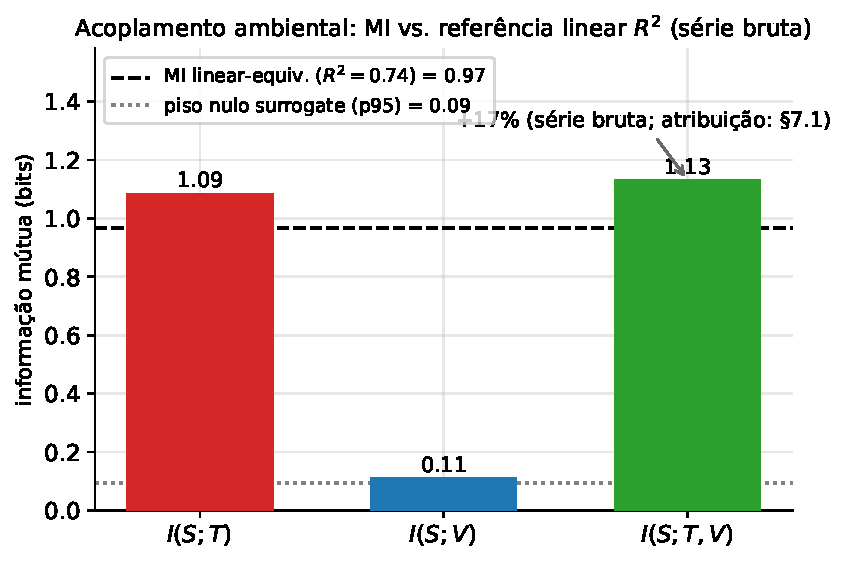
\includegraphics[width=0.86\linewidth]{fig_mi.pdf}
  \caption{Informação mútua por canal e conjunta entre \emph{slack} e o
  ambiente (bits), estimador com \emph{binning}. A conjunta
  $\MI{\slk}{\Tdie,\Vcore}$ excede a Gaussiana-equivalente do $R^2$ linear
  (tracejado) em $\valMIexcessPctBinned\%$ (KSG: $\valMIexcessPctKSG\%$), e
  fica bem acima do piso nulo \emph{surrogate} (pontilhado), confirmando
  acoplamento genuíno (a atribuição do excesso à não-linearidade é
  discutida na \cref{sec:discussion}).}
  \label{fig:mi}
\end{figure}

% Tabela principal: medidas de informação vs. a referência linear R^2.
\begin{table}[t]
  \centering
  \caption{Medidas de informação (bits) vs.\ a referência linear $R^2$ na
           campanha PID. A $\MI{\slk}{\Tdie,\Vcore}$ medida excede a MI
           Gaussiana-equivalente do ajuste linear
           ($-\tfrac12\log_2(1-R^2)$) em \valMIexcessPct\,\% --- um excesso
           real (sobrevive ao piso de viés do estimador), cuja atribuição à
           não-linearidade instantânea, porém, não sobrevive à remoção da
           tendência compartilhada (\cref{sec:res-mi,sec:discussion}). As
           colunas de trabalho anterior são as estatísticas publicadas de
           fidelidade térmica.}
  \label{tab:mi_vs_r2}
  \begin{tabular}{lccc}
    \toprule
     & PID (nova execução) & PID (anterior) & Bang-bang (anterior) \\
    \midrule
    $R^2$ linear $(\slk\mid\Tdie,\Vcore)$       & \valRsqLinear & \valRsqPid & \valRsqBangBang \\
    \;$\hookrightarrow$ MI Gaussiana-equiv.\ (bits) & \valMIlinEquiv & --- & --- \\
    $\Ent{\slk}$ (bits)                      & \valHs        & ---        & --- \\
    $\Ent{\slk\mid\Tdie,\Vcore}$ (bits)      & \valHscondTV  & ---        & --- \\
    $\MI{\slk}{\Tdie}$ (bits)                & \valMIst      & ---        & --- \\
    $\MI{\slk}{\Vcore}$ (bits)               & \valMIsv      & ---        & --- \\
    $\MI{\slk}{\Tdie,\Vcore}$ com \emph{binning} (bits)  & \valMIstv     & ---        & --- \\
    \;$\hookrightarrow$ verificação cruzada KSG (bits) & \valKSGstv  & ---        & --- \\
    \;$\hookrightarrow$ IC 95\,\% (bootstrap em blocos) & [\valMIciLo,\,\valMIciHi] & --- & --- \\
    fração de informação $\MI{}{}/\Ent{}$         & \valInfoFraction & ---     & --- \\
    \bottomrule
  \end{tabular}
\end{table}


\subsection{Correção PVT como recuperação de informação}
\label{sec:res-correction}
Ajustamos $\hat{\dpvt}(\Tdie,\Vcore)$ e formamos $\scorr=\slk-\hat{\dpvt}$. A
correção por mínimos quadrados ordinários (linear) zera o acoplamento linear
por construção ($\operatorname{corr}(\scorr,\Tdie)=+0.00$,
$\operatorname{corr}(\scorr,\Vcore)=-0.00$); a pergunta metodologicamente
relevante é quanta informação mútua \emph{reversível} ela remove. Medido
sobre sinais detrendizados --- para que a deriva lenta de envelhecimento não
se disfarce de acoplamento ambiental --- o acoplamento reversível cai de
$\valPreMIrev$~bits antes da correção para $\valResidMI$~bits depois, ou
seja, a correção linear remove \textbf{\valMIreductionPct\,\%} da informação
reversível ambiente--sensor, deixando um resíduo no piso de ruído do
estimador. O desvio-padrão residual reversível é $\valResidSigmaLin$~contagens,
consistente com o resíduo PID publicado no trabalho anterior
($\valResidPid$~contagens) --- uma verificação cruzada independente do
\emph{pipeline}.

A correção não-linear motivada pela física (tipo Arrhenius em $\Tdie$,
super-linear em $\Vcore$) remove marginalmente mais MI residual
($\valResidMInl$ vs.\ $\valResidMIlin$~bits), mas reduz a variância residual
de forma negligenciável; o critério MDL/BIC (\cref{eq:mdl},
\cref{sec:th-mdl}) portanto \textbf{seleciona o modelo linear}
($\valCorrModel$), julgando os parâmetros extras injustificados neste ponto
de estresse --- um veredito de comprimento de descrição revisitado na
\cref{sec:discussion}.

\paragraph{Recuperação do envelhecimento (resultado-chave).} Remover a
contribuição PVT não apenas limpa o sinal --- ela \emph{expõe} a trajetória
latente de envelhecimento. A correlação do \emph{slack} com o tempo se
fortalece de $\operatorname{corr}(\slk,\tm)=\valCorrStRaw$ no fluxo bruto
para $\operatorname{corr}(\scorr,\tm)=\valCorrStCorr$ após a correção:
retirar a informação ambiental reversível torna a deriva permanente de
envelhecimento a estrutura dominante no resíduo, precisamente o objetivo de
recuperação de informação da \cref{eq:model} e a âncora empírica para o
limite de RUL da \cref{sec:res-rul}.

\begin{figure}[t]
  \centering
  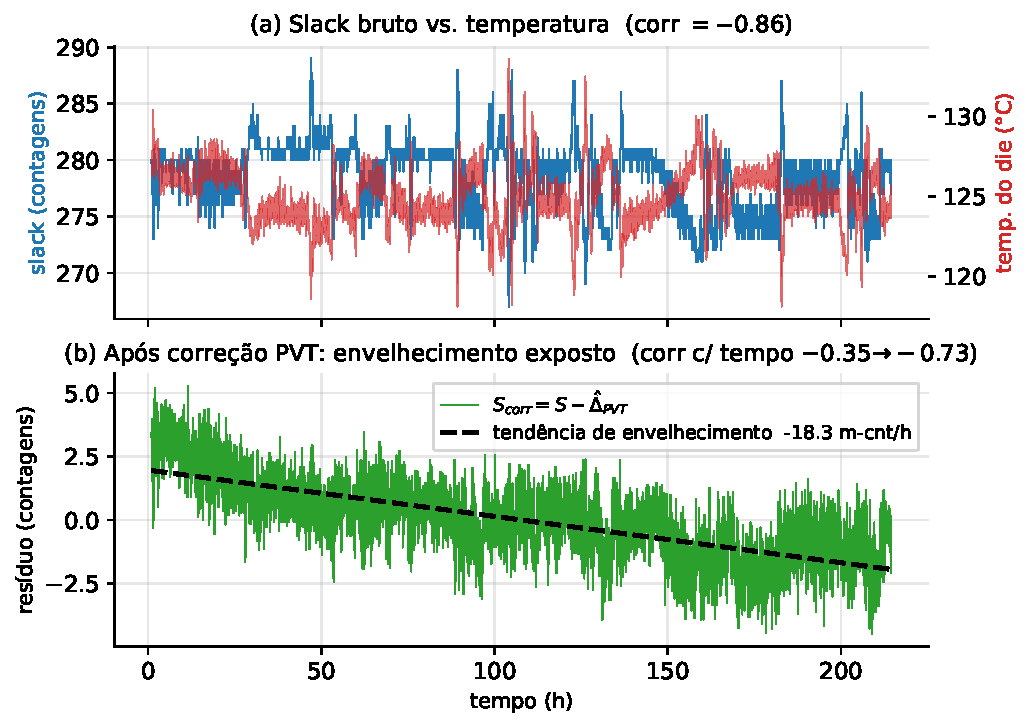
\includegraphics[width=\linewidth]{fig_correction.pdf}
  \caption{(a) O \emph{slack} bruto acompanha a temperatura do \emph{die}
  (corr $\valCorrST$). (b) Após a correção PVT o acoplamento reversível
  desaparece e a tendência permanente de envelhecimento é \emph{exposta}
  (a correlação \emph{slack}--tempo se fortalece de $\valCorrStRaw$ para
  $\valCorrStCorr$); a linha tracejada é a taxa de envelhecimento ajustada.}
  \label{fig:correction}
\end{figure}

\subsection{Distância distribucional entre bancadas}
\label{sec:res-kl}
Duas execuções estabilizadas de $\sim$24~h em bancadas diferentes --- a
configuração SBCCI não-PID e a referência controlada por PID --- permitem
colocar um número em ``quão longe o ambiente não-conforme empurra a
distribuição do \emph{slack}''. Ambas as execuções são no mesmo dispositivo
de teste dedicado, distinto do dispositivo de envelhecimento de 214~h das
seções anteriores; elas compartilham esse dispositivo de teste, de modo que
a divergência isola a diferença de bancada/ambiente e não a variação
dispositivo-a-dispositivo. As bancadas operam em pontos de operação
diferentes, então a comparação é feita sobre a flutuação centrada do
\emph{slack}, isolando o caráter do ruído do ponto de ajuste. O ruído de
\emph{slack} é de $\valSlackStdSBCCI$ contagens (SBCCI) vs.\
$\valSlackStdPID$ contagens (PID), acompanhando o ruído de temperatura
($\valTstdSBCCI$ vs.\ $\valTstdPID$~$^\circ$C) --- a contaminação é de
origem térmica.

A divergência de Kullback--Leibler é fortemente \emph{assimétrica}:
$\KL{p_{\text{SBCCI}}}{p_{\text{PID}}}=\valKLsp$~bits (o custo de descrever a
bancada ruidosa com a referência PID apertada) contra
$\KL{p_{\text{PID}}}{p_{\text{SBCCI}}}=\valKLps$~bits --- uma ilustração
direta do ponto da disciplina de que KL não é uma métrica. A divergência de
Jensen--Shannon, simétrica, é $\valJSbench$~bits (de um máximo de 1), uma
única ``distância entre ambientes de validação'' transferível. Uma forma
fechada Gaussiana de média nula dá $\valKLgauss$~bits para
$\KL{p_{\text{SBCCI}}}{p_{\text{PID}}}$; o valor empírico é maior
($\valKLsp$~bits), e esse excesso é, por si só, evidência de que a bancada
não-conforme injeta excursões \emph{não-Gaussianas}, de cauda pesada --- o
que motiva a análise de separação cega da \cref{sec:res-ica}.

\begin{figure}[t]
  \centering
  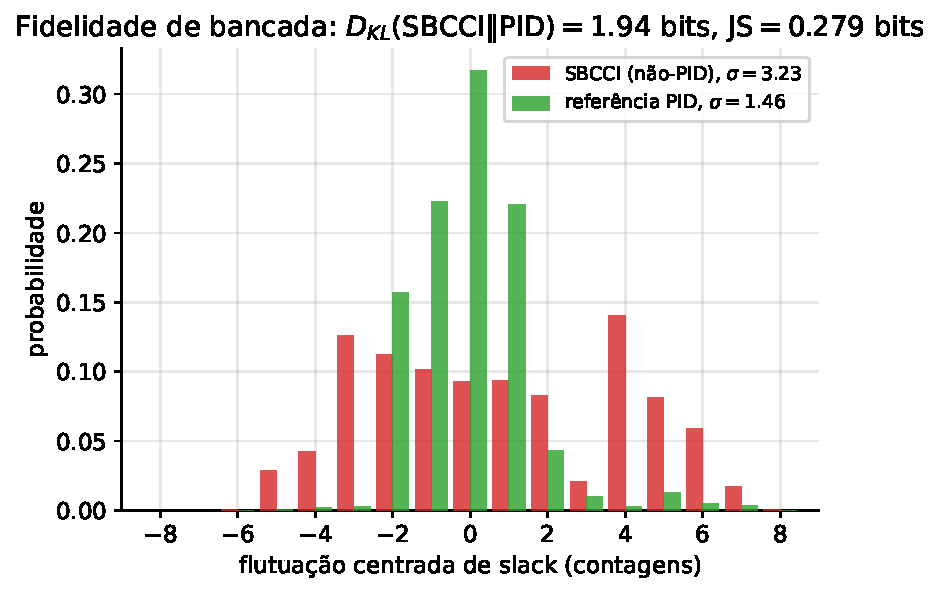
\includegraphics[width=0.86\linewidth]{fig_kl.pdf}
  \caption{Distribuições da flutuação centrada de \emph{slack} das duas
  bancadas (mesmo dispositivo de teste). A bancada SBCCI não-PID é
  marcadamente mais larga que a referência PID; a divergência
  $\KL{p_{\text{SBCCI}}}{p_{\text{PID}}}=\valKLsp$~bits (JS $=\valJSbench$~bits)
  quantifica a lacuna de fidelidade de bancada.}
  \label{fig:kl}
\end{figure}

\subsection{Resolução efetiva e confiabilidade de alarme}
\label{sec:res-capacity}
Tomando o ruído reversível pós-correção $\sigma_{\text{noise}}=\valSigNoise$
contagens e a dispersão do sinal de envelhecimento
$\sigma_{\text{sig}}=\valSigSignal$ contagens, a heurística de capacidade
(\cref{eq:capacity}, derivada na \cref{sec:th-capacity} a partir do
argumento de entropia máxima Gaussiana) dá $\mathrm{SNR}=\valSNR$,
$C=\valCapacityBits$~bits e, portanto, \valCapacityStates{} estados de
envelhecimento distinguíveis ao longo desta campanha --- um número
deliberadamente modesto, que reflete uma excursão de envelhecimento de
apenas $\sim\!\sqrt{\valSNR}\times$ o piso de ruído, e que a métrica
residual-$\sigma$ anterior não conseguia expressar.

A decisão de alarme de envelhecimento é modelada como um BSC cujo
cruzamento $p$ decorre do SNR de detecção por janela (\cref{eq:bsc}). A
confiabilidade é fortemente \emph{dependente da escala de tempo}: uma
decisão por hora é essencialmente um lançamento de moeda ($p\approx0.49$,
$\Cbsc\approx0$) porque uma hora de deriva está enterrada no ruído, enquanto
uma janela operacional de \valBSCwindow~h dá $p=\valBSCp$ e
$\Cbsc=\valBSCcap$~bits/decisão (quase perfeito), e a campanha completa é
efetivamente certa. A transição entre esses regimes coincide com o tempo
mínimo de observação derivado a seguir.

\begin{figure}[t]
  \centering
  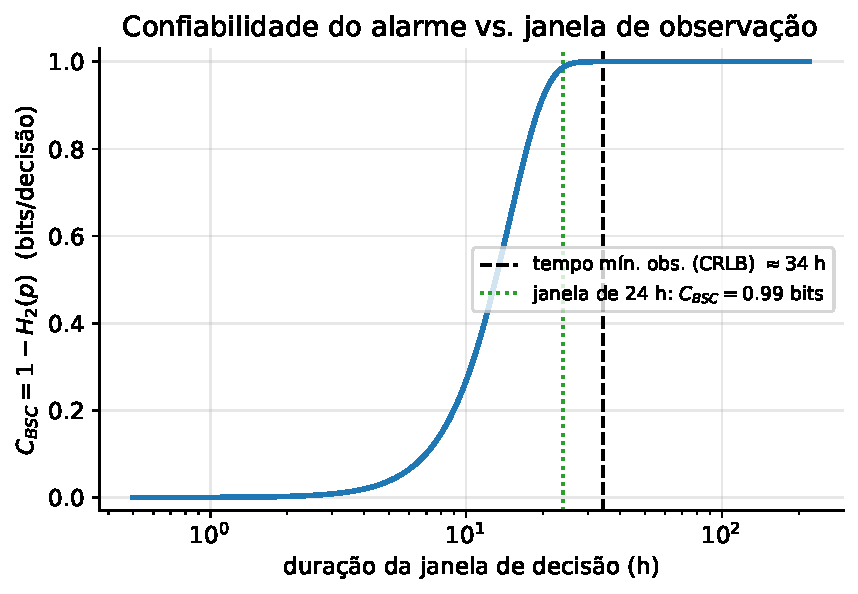
\includegraphics[width=0.82\linewidth]{fig_capacity_rul.pdf}
  \caption{Capacidade do canal de alarme de envelhecimento
  $\Cbsc=1-\Hb(p)$ em função do comprimento da janela de decisão. A
  confiabilidade sobe de $\approx0$ (por hora, enterrada no ruído) para
  $\approx1$ bit, com a transição coincidindo com o tempo mínimo de
  observação de Cram\'er--Rao ($\approx\valMinObsTime$~h, tracejado) --- as
  três figuras de mérito são mutuamente consistentes.}
  \label{fig:capacity}
\end{figure}

\subsection{Limite de detectabilidade de RUL}
\label{sec:res-rul}
Colocando o RUL como estimação por mínimos quadrados da inclinação de
envelhecimento, e usando o ruído medido com o tamanho efetivo de amostra
$\neff=\valNeff$ ($\tauint=\valTauInt$~amostras, ou seja,
$\sim$5~min de decorrelação), o limite de Cram\'er--Rao
(\cref{sec:th-estimation}) dá um desvio-padrão da estimativa de inclinação
de $\valCRLBsd$~m-cnt/h ao longo da campanha de $\sim$214~h, portanto uma
taxa mínima detectável de envelhecimento (a $3\sigma$) de
\textbf{\valMinDetectRate~m-cnt/h}. A taxa de envelhecimento corrigida
medida é $\valAgingSlope$~m-cnt/h --- aproximadamente $15\times$ acima desse
piso, de modo que a tendência é firmemente detectável. Equivalentemente, o
tempo mínimo de observação para resolver a tendência medida a $3\sigma$ é
\textbf{$\sim$\valMinObsTime~h}, bem dentro desta campanha (e explicando por
que as execuções anteriores de $\sim$23~h não conseguiam separar o
envelhecimento do piso reversível). Esta é a afirmação honesta de
detectabilidade que o projeto prometeu: não uma predição de vida útil, mas
um limite limitado por ruído sobre \emph{quando} o envelhecimento se torna
observável.

\paragraph{Barras de credibilidade Bayesianas.} O limite frequentista é
complementado por uma regressão linear Bayesiana de $\scorr$ sobre o tempo,
ajustada sobre os dados decimados até os $\neff$ pontos efetivamente
independentes (para que a verossimilhança i.i.d.\ seja válida) sob uma
\emph{prior} de Jeffreys, dando uma posterior $t$ de Student para a
inclinação. A taxa de envelhecimento posterior é $\valBayesSlope$~m-cnt/h
com um intervalo de credibilidade de $95\%$ de
$[\valBayesSlopeLo,\valBayesSlopeHi]$~m-cnt/h, e a probabilidade posterior de
que a inclinação seja genuinamente negativa é de $\valBayesPaging\,\%$ ---
numericamente indistinguível de certeza; a leitura dessa deriva residual
\textbf{como envelhecimento} permanece condicionada à hipótese de
identificação deste estudo de dispositivo único (\cref{sec:discussion},
ameaças à validade). Propagar a posterior da inclinação pela relação de detectabilidade
dá um intervalo de credibilidade de $[\valBayesMotLo,\valBayesMotHi]$~h para
o tempo mínimo de observação, contendo a estimativa pontual de
$\valMinObsTime$~h. Os dois paradigmas concordam, e o tratamento Bayesiano
fornece as barras de erro calibradas que um futuro estudo de RUL propagaria
adiante.

\subsection{Uma trajetória de envelhecimento denoised e o RUL como distribuição (Wiener/Kalman)}
\label{sec:res-wiener}
Os resultados de Cram\'er--Rao e Bayesiano acima fornecem uma única taxa
para toda a campanha e sua barra de erro. Aqui fazemos, em vez disso, a
pergunta de estimação sequencial da \cref{sec:th-wiener}: fazendo a média em
blocos de $\scorr$ em $\valNBlocks$ observações quase-independentes (uma a
cada $2\tauint$, ou seja, uma unidade de $\neff$ cada), o ajuste por método
dos momentos da \cref{eq:wiener-model} dá uma difusão de Wiener
$\sigma_B=\valWienerSigmaB$ contagens/$\sqrt{\text{h}}$ e um ruído de
observação por média de bloco $R$ notavelmente \emph{abaixo} do
$\sigma_{\text{noise}}^2$ nativo por amostra (\cref{sec:res-capacity}) ---
evidência direta de que a média sobre uma janela completa de decorrelação
ainda remove estrutura sub-$\tauint$ que o tempo de autocorrelação único,
sozinho, não captura. O MLE do ruído de taxa colapsa para seu piso numérico
($\sigma_{\mathrm{rate}}^2\!\approx\!\valWienerQRate$): os dados preferem um
processo de Wiener de deriva \emph{constante} a um variável no tempo, uma
segunda confirmação independente --- ao lado do veredito de MDL da
\cref{sec:res-correction} --- de que esta campanha única, de ponto de
operação estreito, não contém informação de curvatura suficiente para
sustentar um modelo mais flexível. A taxa suavizada por Kalman/RTS ao final
da campanha é $\valWienerRateEnd$~m-cnt/h, consistente em sinal e ordem de
grandeza com a estimativa CRLB/Bayesiana da \cref{sec:res-rul}
($\sim\!-18$~m-cnt/h); a diferença de $\sim$15\% entre as duas taxas
derivadas independentemente reflete os estimadores distintos (OLS sobre toda
a série vs.\ um estado filtrado, com média em blocos), não uma contradição.
O desvio-padrão posterior do nível suavizado é essencialmente plano ao longo
da campanha ($\valWienerLevelSDstart\to\valWienerLevelSDend$ contagens): o
filtro atinge sua incerteza de regime permanente dentro dos primeiros
blocos e não continua encolhendo indefinidamente, exatamente como um filtro
linear-Gaussiano com $R$ e $\sigma_B^2$ constantes prevê.

\begin{figure}[t]
  \centering
  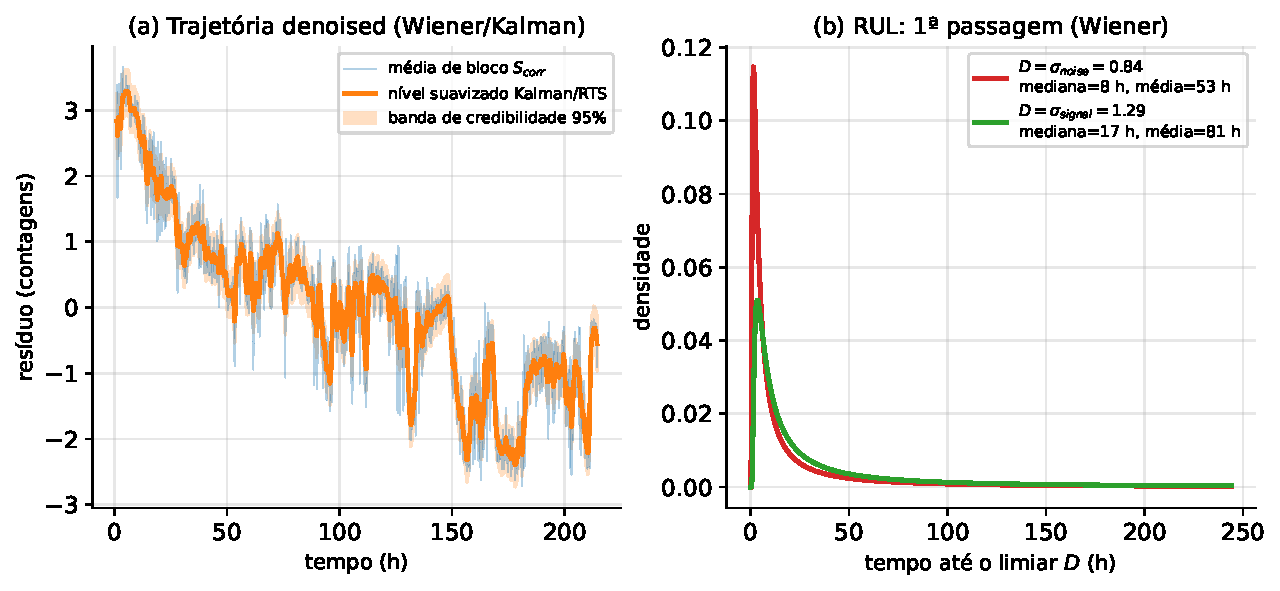
\includegraphics[width=\linewidth]{fig_wiener_rul.pdf}
  \caption{(a) Média de bloco de $\scorr$ (claro) e a trajetória de
  envelhecimento suavizada por Kalman/RTS $\hat\Xlat(t)$ com uma banda de
  credibilidade de 95\%. (b) A distribuição de RUL Gaussiana-inversa
  (\cref{eq:invgauss}) em dois limiares ancorados no Tier 1: um incremento
  do piso de ruído ($D=\sigma_{\text{noise}}$) e uma excursão em escala de
  sinal já observada ($D=\sigma_{\text{signal}}$).}
  \label{fig:wiener}
\end{figure}

\paragraph{RUL como distribuição.} Em $D=\sigma_{\text{noise}}=\valDnoise$
contagens (o mesmo piso de ruído que limita o sensor a
\valCapacityStates{} estados distinguíveis, \cref{sec:res-capacity}), o
tempo de primeira passagem de Wiener tem média $\valRULmeanNoise$~h mas
mediana $\valRULmedianNoise$~h; em $D=\sigma_{\text{signal}}=\valDsignal$
contagens, média $\valRULmeanSignal$~h e mediana $\valRULmedianSignal$~h. A
grande diferença entre média e mediana em ambos os casos não é um artefato:
a Gaussiana inversa é fortemente assimétrica à direita exatamente quando o
limiar $D$ é pequeno em relação à escala de difusão $\sigma_B$, que é
precisamente o regime de SNR baixo ($\mathrm{SNR}=\valSNR$,
\cref{sec:res-capacity}) medido aqui --- \emph{a mesma limitação de ruído
que restringe os estados resolvíveis do sensor também torna as predições de
RUL de curto horizonte altamente incertas}, uma ligação quantitativa entre o
resultado de capacidade e o resultado de RUL que uma única estimativa
pontual não consegue expressar. Isso é oferecido como uma
\emph{metodologia} para uma distribuição completa de RUL, exercitada em
limiares auto-referenciados porque, como em todo este trabalho, não existe
um limiar de falha calibrado externamente para este sensor; fornecer um
(\cref{sec:conclusion}) transforma a \cref{eq:invgauss} diretamente em uma
distribuição de RUL operacional.

\subsection{Separação cega de fontes (ICA)}
\label{sec:res-ica}
Como contraparte livre de modelo à correção por regressão da
\cref{sec:res-correction}, o FastICA \cite{hyvarinen2001} (contraste de
negentropia, \cref{eq:negentropy} na \cref{sec:th-ica}) foi aplicado aos três canais
observados $(\slk,\Tdie,\Vcore)$ isoladamente, sem nenhuma forma funcional
assumida para $\dpvt$. O componente recuperado que acompanha o tempo bate
com o resíduo de envelhecimento baseado em regressão $\scorr$ em
$|\mathrm{corr}|=\valICAagingScorr$ --- \emph{o ICA livre de modelo chega
independentemente a essencialmente o mesmo sinal de envelhecimento que a
regressão produziu}, o que valida cruzadamente a correção PVT sem usar o
acoplamento medido $\Tdie,\Vcore$. Um segundo componente se alinha com a
temperatura ($|\mathrm{corr}(\cdot,\Tdie)|=\valICAthermalT$). Ambas as
fontes recuperadas são fortemente não-Gaussianas (curtose em excesso
$\valICAkurtAging$ e $\valICAkurtThermal$), confirmando a premissa de que a
não-Gaussianidade é a característica que distingue as fontes físicas --- e
consistente com as excursões de cauda pesada que a análise KL
(\cref{sec:res-kl}) expôs.

A separação é \emph{parcial}, e é reportada como tal: a informação mútua
residual entre pares de componentes recuperados atinge $\valICAresidMI$~bits
(a independência ideal é $0$), porque a deriva lenta e não-estacionária de
envelhecimento e o ruído de cauda pesada satisfazem apenas
aproximadamente as hipóteses de i.i.d./estacionariedade do ICA. O ICA é,
portanto, corroborativo aqui --- uma rota independente, com poucas hipóteses,
para o mesmo componente de envelhecimento --- em vez de uma desmistura
limpa. O ICA recebe os três mesmos canais observados $(\slk,\Tdie,\Vcore)$ da
regressão e busca no mesmo espaço linear de 3 dimensões; a diferença está no
\emph{critério}, não no espaço de busca --- mínimos quadrados de um lado,
independência/não-Gaussianidade (negentropia) do outro. Que dois critérios
tão distintos, aplicados às mesmas observações, cheguem a componentes de
envelhecimento com $|\mathrm{corr}|=\valICAagingScorr$ (isto é,
$\approx\valICAagingVarExpl\,\%$ de variância compartilhada --- não
$\valICAagingVarExpl\,\%$ do ``sinal recuperado'', uma leitura que confundiria
correlação com fração de sinal) é, ainda assim, uma corroboração de critério
não trivial.

\begin{figure}[t]
  \centering
  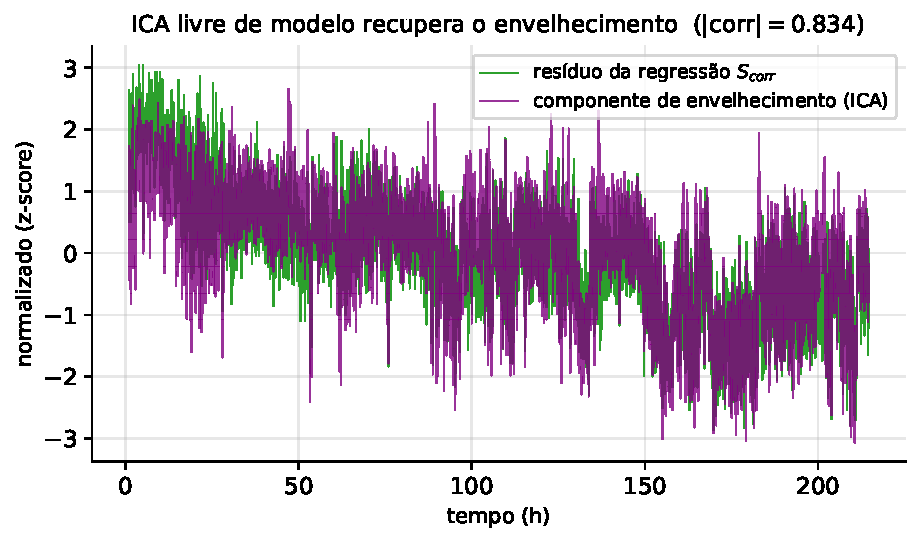
\includegraphics[width=\linewidth]{fig_ica.pdf}
  \caption{O componente de envelhecimento recuperado pelo ICA (roxo)
  sobreposto ao resíduo baseado em regressão $\scorr$ (verde), ambos
  padronizados ($z$-score). O ICA livre de modelo, dado apenas
  $(\slk,\Tdie,\Vcore)$, acompanha o sinal de envelhecimento da regressão em
  $|\mathrm{corr}|=\valICAagingScorr$.}
  \label{fig:ica}
\end{figure}

%==============================================================================
\section{Discussão}
\label{sec:discussion}

% --- corresponde a 01_Project_Overview.md §6 (contribuição) e §7 (ressalvas) ---

\subsection{O que a teoria da informação acrescenta sobre $R^2$}
Uma métrica de ruído correta e transferível: a informação mútua não assume
uma forma funcional, é válida onde a física é não-linear e é expressa em
bits, ao contrário da fração de variância. Sobre a série bruta --- o
pareamento correto com o $R^2$ publicado do trabalho anterior, também
medido sobre série bruta --- a dependência medida excede o equivalente
linear-$R^2$ em $\valMIexcessPctBinned$--$\valMIexcessPctKSG\,\%$. Esse
excesso é real (sobrevive ao piso de viés do estimador,
\cref{sec:res-mi}), mas \textbf{não é, por si só, evidência de
não-linearidade instantânea na relação reversível $\Tdie,\Vcore\to\slk$}: a
mesma comparação sobre as séries detrendizadas mostra um \emph{déficit}, não
um excesso ($\valMIexcessPctDetrended\,\%$, \cref{sec:res-mi}), de modo que
o excesso bruto está concentrado na tendência lenta que envelhecimento e
$\Tdie,\Vcore$ compartilham ao longo da campanha, não na física
Arrhenius/BTI instantânea que motivou este projeto. A contribuição
metodológica --- MI em vez de $R^2$ como a métrica correta e transferível,
válida mesmo quando a forma da dependência é desconhecida --- permanece de
pé; a interpretação causal específica (``a MI excede o $R^2$ porque a
física subjacente é não-linear'') não é sustentada por este resultado e é
retirada. Isso também enfraquece a extrapolação entre regimes térmicos: mesmo a
leitura mais cautelosa --- que a comparação anterior, baseada em $R^2$,
entre bang-bang e PID poderia subestimar a diferença real entre eles ---
perde parte de sua base, já que o excesso não-linear que a sustentaria não
se mostrou robusto ao \emph{detrend}; recalcular ambas as bancadas lado a
lado em bits exigiria, de qualquer forma, uma execução pareada no mesmo
dispositivo em ambos os regimes, fora do escopo deste estudo de regime
único (\cref{sec:discussion}, ameaças à validade).

\subsection{Uma definição principiada de qualidade de \emph{burn-in}}
Reenquadrar a qualidade de \emph{burn-in} como a minimização de
$\MI{\slk}{\Tdie,\Vcore}$ dá à afirmação qualitativa ``PID é um ambiente de
validação mais limpo'' uma unidade rigorosa e um alvo de otimização: cada
bit que o ambiente escreve na leitura de \emph{slack} é um bit de
informação de envelhecimento perdido. Enunciamos isso como um princípio, em
vez de demonstrá-lo dentro de um único dispositivo; o suporte empírico mais
próximo aqui é a lacuna distribucional entre as duas bancadas
(\cref{sec:res-kl}), medida em um dispositivo de teste separado.

\subsection{Uma visão por comprimento de descrição da escolha linear-vs-não-linear}
O critério MDL da \cref{sec:th-mdl}, que seleciona a correção PVT linear
(\cref{sec:res-correction}), não é uma penalidade \emph{ad hoc} sobre
parâmetros extras: é um substituto computável para a intuição de
complexidade de Kolmogorov de que o melhor modelo é a \emph{descrição mais
curta} que ainda explica os dados (\cref{eq:kolmogorov}). Enquadrado dessa
forma, o resultado não é meramente ``a correção não-linear não vale a pena
aqui'' --- é que, neste único e estreito ponto de operação
(\valDutTempMean~$^\circ$C, \valDutVoltMean~V), os dados ainda não contêm
informação de curvatura suficiente para justificar pagar pelos parâmetros
extras do modelo Arrhenius/super-linear, mesmo que a física subjacente seja
genuinamente não-linear (\cref{sec:background-r2}). Isso é, na verdade,
\textbf{a mesma conclusão} alcançada por uma rota independente: o excesso
de MI sobre o equivalente Gaussiano linear, que motivou este projeto, não
sobrevive quando medido sobre o acoplamento reversível detrendizado
(\cref{sec:res-mi}). MDL (nesta seção) e a checagem de MI detrendizada
(\cref{sec:res-mi}) perguntam coisas diferentes --- se uma forma paramétrica
não-linear específica se paga na correção, e se o acoplamento reversível
\emph{instantâneo} contém excesso de dependência não-linear, respectivamente
--- mas os dois, de forma independente, dizem que este conjunto de dados de
único ponto de operação não contém evidência de não-linearidade
\emph{instantânea} entre $\Tdie,\Vcore$ e $\slk$, mesmo que a física
subjacente seja genuinamente não-linear em uma faixa mais ampla de operação.
Uma campanha de faixa mais larga ou com múltiplos pontos de ajuste, cobrindo
curvatura Arrhenius/BTI suficiente para ser compressível pelo modelo
não-linear, é a condição natural sob a qual ambos os vereditos se
inverteriam.

\subsection{Um limite de resolução para sensores de SLM}
Os resultados de capacidade e BSC colocam números concretos sobre o que o
sensor consegue fazer: \valCapacityStates{} estados de envelhecimento
distinguíveis ao longo da campanha, um alarme diário
($\valBSCwindow$~h) de envelhecimento de $\Cbsc=\valBSCcap$~bits, e um piso
de detecção a $3\sigma$ de \valMinDetectRate~m-cnt/h atingido após
$\sim$\valMinObsTime~h. Isso informa a um projetista de SLM quão finamente o
sensor resolve o envelhecimento e quão confiavelmente ele pode disparar um
alarme sob ruído realista --- grandezas diretamente consumidas por
escalonamento adaptativo de tensão e RUL, e que a métrica residual-$\sigma$
anterior deixava implícitas. Sua consistência mútua (a confiabilidade do
BSC por janela cruza próximo ao tempo mínimo de observação do CRLB) é
evidência de que o modelo de canal é coerente, e não três heurísticas
desconectadas.

\subsection{Estimação sequencial e RUL como distribuição}
O tratamento Wiener/Kalman da \cref{sec:res-wiener} deliberadamente não é um
substituto do limite de Cram\'er--Rao/Bayesiano da \cref{sec:res-rul}, mas
uma verificação cruzada a partir de uma rota de estimação independente (um
modelo dinâmico e filtrado, em vez de uma única regressão sobre toda a
série) que, por sinal, concorda no sinal e na ordem de grandeza da taxa de
envelhecimento. Seu valor agregado é estrutural, não numérico: transforma
uma única taxa pontual com barra de erro em (i) uma estimativa de
trajetória denoised, continuamente atualizada, que o operador poderia, em
princípio, consumir on-line, e (ii) uma \emph{distribuição} completa de RUL,
em vez de um limite, expondo a assimetria à direita que uma barra de erro
Gaussiana esconde. O fato de que o MLE do ruído de taxa e o critério MDL da
\cref{sec:res-correction} \emph{independentemente} preferem, ambos, o modelo
mais simples disponível (deriva constante; correção linear) neste único
ponto de operação é, por si só, um achado: dois princípios de estimação
diferentes, aplicados a duas perguntas diferentes, concordam que esta
campanha ainda não contém a curvatura necessária para justificar um modelo
mais flexível --- exatamente o tipo de validação cruzada que este projeto
usou ao longo de todo o trabalho (KSG vs.\ MI com \emph{binning},
frequentista vs.\ RUL Bayesiano, ICA vs.\ correção por regressão).

\subsection{Ameaças à validade}
O excesso de informação mútua sobre o equivalente Gaussiano-linear, medido
na série bruta (\cref{sec:res-mi}), não sobrevive à remoção da tendência de
envelhecimento compartilhada e não deve ser lido como demonstração de
não-linearidade instantânea na física PVT reversível --- esse é o achado
mais importante desta seção de ameaças à validade, não uma nota de rodapé,
e é discutido em detalhe nas \cref{sec:res-mi,sec:discussion}. A análise do
dispositivo de envelhecimento é de um único dispositivo e um
único regime térmico, o que limita a separabilidade do envelhecimento
permanente. A comparação de bancadas da \cref{sec:res-kl} é em um
dispositivo de teste \emph{diferente}, de modo que sua divergência KL/JS
fala sobre a fidelidade de bancada, e não sobre o comportamento do
dispositivo de envelhecimento, e os dois nunca são misturados. Estimativas
de MI em dados autocorrelacionados são propensas a viés, apesar da grande
contagem bruta de amostras, mitigado (não eliminado) por $\neff$, pelo piso
nulo \emph{surrogate} da \cref{sec:res-mi} e pela comparação entre
estimadores independentes (\emph{binning} vs.\ KSG), cuja diferença
sistemática é reportada como faixa de incerteza, não escondida; a
expressão de capacidade é uma heurística de resolução
efetiva; a separação por ICA é corroborativa, não uma desmistura limpa. O
modelo Wiener/Kalman da \cref{sec:res-wiener} assume ruído de observação por
média de bloco constante e um processo latente genuinamente difusivo
(Wiener); a distribuição de RUL que ele produz é reportada em limiares
auto-referenciados, já calculados, precisamente porque não existe um limiar
de falha calibrado de forma independente para este sensor, de modo que é
uma demonstração de \emph{metodologia}, não uma predição operacional de
vida útil, no mesmo espírito do limite de Cram\'er--Rao da
\cref{sec:res-rul}.

%==============================================================================
\section{Conclusão e Trabalhos Futuros}
\label{sec:conclusion}

Colocamos uma camada de medição informacional sobre uma plataforma de
\emph{burn-in} de envelhecimento acelerado já existente, reexpressando a
contaminação ambiental, a correção PVT e a recuperabilidade do
envelhecimento como entropia, informação mútua e capacidade de canal. Em
uma campanha PID de \valDurationHours~h estabelecemos as âncoras empíricas
($\Ent{\slk}=\valHs$~bits; $R^2$ linear $=\valRsqLinear$) e uma metodologia
que substitui o $R^2$ dependente de modelo pela informação mútua, define
qualidade de \emph{burn-in} como a minimização de
$\MI{\slk}{\Tdie,\Vcore}$, converte o ruído medido em estados de
envelhecimento resolvíveis e uma capacidade de canal de alarme, e limita a
detectabilidade de RUL honestamente via Cram\'er--Rao e estimação
Bayesiana. Uma extensão via processo de Wiener e filtro de Kalman do mesmo
ferramental de estimação transforma ainda mais esse limite pontual de RUL
em uma trajetória de envelhecimento denoised, continuamente atualizada, e
uma \emph{distribuição} de RUL Gaussiana-inversa em forma fechada
(\cref{sec:res-wiener}), validada cruzadamente contra a estimativa
CRLB/Bayesiana e contra o resultado de seleção de modelo por MDL da
\cref{sec:res-correction}.

A proposta original deste projeto previa uma estimativa de capacidade
\emph{por regime térmico} (\emph{bang-bang} vs.\ PID); sem um registro bruto
de \emph{bang-bang} sincronizado e comparável ao da campanha PID de
\valDurationHours~h, essa comparação por regime não foi entregue como tal
--- em seu lugar, este trabalho entrega a capacidade e o limite de RUL no
regime PID (\cref{sec:res-capacity,sec:res-rul}) e, como sucedâneo direto
para a comparação entre regimes, a divergência distribucional KL/JS entre
as duas bancadas (\cref{sec:res-kl}), que já mostra numericamente que a
bancada não-PID é mais ruidosa. Completar a comparação de capacidade por
regime com um registro \emph{bang-bang} novo é, por isso, o primeiro item
de trabalho futuro abaixo, não uma lacuna silenciosa.

\paragraph{Trabalhos futuros.} Adquirir uma campanha \emph{bang-bang} de
duração equivalente para completar a comparação de KL e capacidade
entre regimes com dados novos; estender para múltiplos dispositivos para
separar uma trajetória de envelhecimento permanente da variação
dispositivo-a-dispositivo; implantar o \emph{pipeline} em janelas
deslizantes, on-line, como um gerador contínuo de atributos informacionais
alimentando o controlador de SLM, com a trajetória suavizada por Kalman da
\cref{sec:res-wiener} como sua estimativa de envelhecimento ao vivo;
calibrar um limiar de falha real $D$ (por exemplo, a partir de uma
especificação de margem de tempo) para que a \cref{eq:invgauss} produza uma
distribuição de RUL operacional, em vez dos limiares auto-referenciados
usados aqui; e prosseguir com a rota de ICA/separação cega com canais
derivados adicionais para fortalecer a recuperação de envelhecimento livre
de modelo.

\section*{Reprodutibilidade}
Todo escalar neste trabalho é gerado pelo \emph{pipeline} de análise em
\texttt{generated/values.tex}, e cada figura/tabela em \texttt{figures/} e
\texttt{tables\_pt/}; reexecutar a análise sobre um novo registro
regenera o documento sem transcrição manual.

\section*{Agradecimentos}
Este trabalho foi desenvolvido para a disciplina de Teoria da Informação
(TIP7266, PPGETI/UFC, 2026.1) e se apoia na pesquisa do autor sobre sensores
de envelhecimento de circuitos integrados e instrumentação de \emph{burn-in}.


\bibliographystyle{IEEEtran}
\bibliography{references}

\end{document}
